% !Mode:: "TeX:UTF-8" 

\BiChapter{基于聚类的克隆代码演化特征分析方法}
{An Analysis for Code Clone Evolutionary Characteristic Based on Clustering Method}

\BiSection{引言}
{Introduction}

复用软件中的既有代码已成为了一种常见的软件开发手段,可以帮助程序开发人员节约开发时间和提高开发效率。然而,复用既有代码会向软件系统中引入大量的克隆代码,即彼此相似的代码片段。在软件随着时间进行演化的过程中,软件系统中的克隆代码不是静止不变的,也会随着软件系统进行演化,研究人员将克隆代码的这一现象称为克隆代码演化。在大量克隆代码及其演化过程中,必然存在着一些隐含的信息可以揭示克隆演化规律,本文将之称为克隆代码演化特征。克隆演化特征不仅可以帮助软件开发人员理解系统中存在的克隆代码,还可以向软件开发人员提供一些如何维护克隆代码的建议。但遗憾的是,当前研究中对克隆演化特征的研究不够充分,缺乏客观且全面的克隆演化特征研究。因此,如何分析并获取克隆代码演化特征是一个值得研究的问题。

为了帮助程序开发人员获得克隆代码演化特征,本章结合机器学习中的聚类分析方法,在提取克隆代码相应度量值表示不同克隆实体的基础上揭示克隆代码演化特征,可以帮助理解和维护克隆代码。首先,为了描述克隆代码的演化过程,本文检测软件系统所有版本的克隆代码,并在此基础上通过映射相邻版本的克隆代码构建软件系统的克隆家系,并扩展和定义了7种不同的克隆演化模式描述克隆代码在演化中的变化情况。然后,从三个不同的角度描述克隆代码及其演化过程,即使用克隆片段、克隆组和克隆家系三种克隆实体。为了使用机器学习方法分析克隆代码及其演化过程,提取了不同度量值分别表示不同的克隆实体。最后,根据所提取的度量值生成相应的聚类向量,并使用聚类分析挖掘和分析克隆代码的演化特征。在开源系统{\em ArgoUML}和{\em jEdit}上进行了实证研究。实验结果表明演化过程中的大部分克隆代码是稳定的,但也存在一定数量的发生变化的克隆代码;在发生变化的克隆代码中,发生一致性变化的克隆代码要多于不一致变化的克隆代码。
%实验结果表明演化过程中的大部分克隆代码是稳定的,不会频繁的发生变化;同时也存在一定数量的发生变化的克隆代码。在发生变化的克隆代码中,发生一致性变化的克隆代码要多于不一致变化的克隆代码。
%因此, 本文建议开发人员应该更加关注寿命较长的克隆代码,同时当克隆代码发生变化时应考虑是否需要将变化传播到同组的克隆代码中从而满足一致性。

\BiSection{克隆演化及其演化特征}
{The Clone Evolution and its Characteristics}

本节介绍与克隆代码演化相关的术语与模型,并给出克隆代码演化特征的定义。

\BiSubsection{克隆代码演化}
{Code Clone Evolution}
\label{ref-evolution}
软件工程实践会产生大量的克隆代码,软件中存在的大量克隆代码不仅使得系统变得更加臃肿,也使得系统越来越难以理解。为收集和检测系统中存在的克隆代码,在过去的20年中,研究人员提出了许多种克隆代码检测方法,并开发了大量的克隆检测工具,例如NiCad\cite{roy2008nicad}、CCFinder\cite{kamiya2002ccfinder}等(有兴趣的读者可以参考本文绪论克隆检测部分~\ref{ref-detection})。目前大多数的克隆检测工具仅可以检测单版本系统中克隆代码,即从系统某一版本的源代码中检测得到克隆代码后,向程序开发人员报告检测结果。克隆检测结果往往以克隆片段和克隆组的形式进行组织,克隆片段是具体克隆代码,克隆组是彼此相似的克隆组的集合。克隆片段和克隆组可以描述如下:\\

\begin{definition} [{克隆片段}]
\label {defn-cf}
克隆片段({\em Clone Fragment, CF})是一段代码片段,包括若干行连续的代码。克隆片段与一些其它的代码片段彼此相似,并将它们称之为彼此相似的克隆片段。
\end {definition}

\begin{definition} [{克隆组}]
\label {defn-cg}
克隆组 ({\em Clone Group, CG})是彼此相似的克隆片段的集合,包含若干个彼此相似的克隆片段。一个克隆组揭示了克隆组内的克隆片段之间的克隆关系。
\end {definition}

%\begin{itemize}
%\item 
%克隆片段:
%克隆片段({\em Clone Fragment, CF})是一段代码片段,包括若干行连续的代码。克隆片段与一些其它的代码片段彼此相似,并将它们称之为彼此相似的克隆片段。
%\item
%克隆组:
%克隆组 ({\em Clone Group, CG})是彼此相似的克隆片段的集合,包含若干个彼此相似的克隆片段。一个克隆组揭示了克隆组内的克隆片段之间的克隆关系。
%\end{itemize}

如绪论所述,克隆代码在系统中不是静止不变的,会随着软件系统的演化同时进行演化。克隆演化过程最早是2001年由Antoniol等人提出,使用时间序列描述克隆代码的演化模型\cite{antoniol2001modeling},但并未引起人们的重视。2005年,Kim提出了克隆家系模型用于描述克隆代码的演化过程,是迄今为止最好的演化模型\cite{kim2005empirical}。本文也使用Kim提出的演化模型描述克隆代码演化过程。克隆代码在演化过程中可能会发生变化,为了描述这种克隆组的变化情况,同时定义克隆演化模式描述克隆代码在演化过程中的变化情况。克隆家系及其演化模式可以描述如下:\\

\begin{definition} [{克隆家系}]
\label {defn-cg}
克隆家系 ({\em Clone Genealogy, CGE})是一个有向无环图,描述了一个克隆组($CG$)随系统进行演化的情况。CGE图中的节点表示系统某一个版本($V_i$)中的该克隆组($CG_i$)。CGE图中的边表示该克隆组($CG$)在相邻的两个版本中$(V_{i-1},V_i )$的演化关系$(CG_{i-1},CG_{i})$,即$CG$由上一版本$V_{i-1}$的$CG_{i-1}$演化至下一版本$V_{i-1}$中的$CG_{i}$。
\end{definition} 

\begin{definition} [{克隆演化模式}]
\label {defn-cep}
克隆演化模式 ({\em Clone Evolution Pattern, CEP})是某一克隆组在演化中的相邻两个版本的演化情况,用于描述该克隆组的变化情况,根据不同的变化具有不同的演化模式。
\end{definition} 

%\begin{itemize}
%\item 
%克隆家系:
%克隆家系 ({\em Clone Genealogy, CGE})是一个有向无环图,描述了一个克隆组($CG$)随系统进行演化的情况。CGE图中的节点表示系统某一个版本($V_i$)中的该克隆组($CG_i$)。CGE图中的边表示该克隆组($CG$)在相邻的两个版本中$(V_{i-1},V_i )$的演化关系$(CG_{i-1},CG_{i})$,即$CG$由上一版本$V_{i-1}$的$CG_{i-1}$演化至下一版本$V_{i-1}$中的$CG_{i}$。
%\item
%克隆演化模式:
%克隆演化模式 ({\em Clone Evolution Pattern, CEP})是某一克隆组在演化中的相邻两个版本的演化情况,用于描述该克隆组的变化情况,根据不同的变化具有不同的演化模式。
%\end{itemize}

为了更为形象的描述克隆家系及其演化模式,本文给出一个克隆家系的示意图,如图~\ref{genealogy}所示。从图中可以看出,克隆家系(CGE)是克隆组(CG)演化的有向无环图,图的节点表示克隆组,图中边表示克隆组的演化关系和演化模式。图~\ref{genealogy}给出一个克隆组在五个版本$(V_i, V_{i+4})$中的演化过程。

\begin{figure}[htbp]
\centering
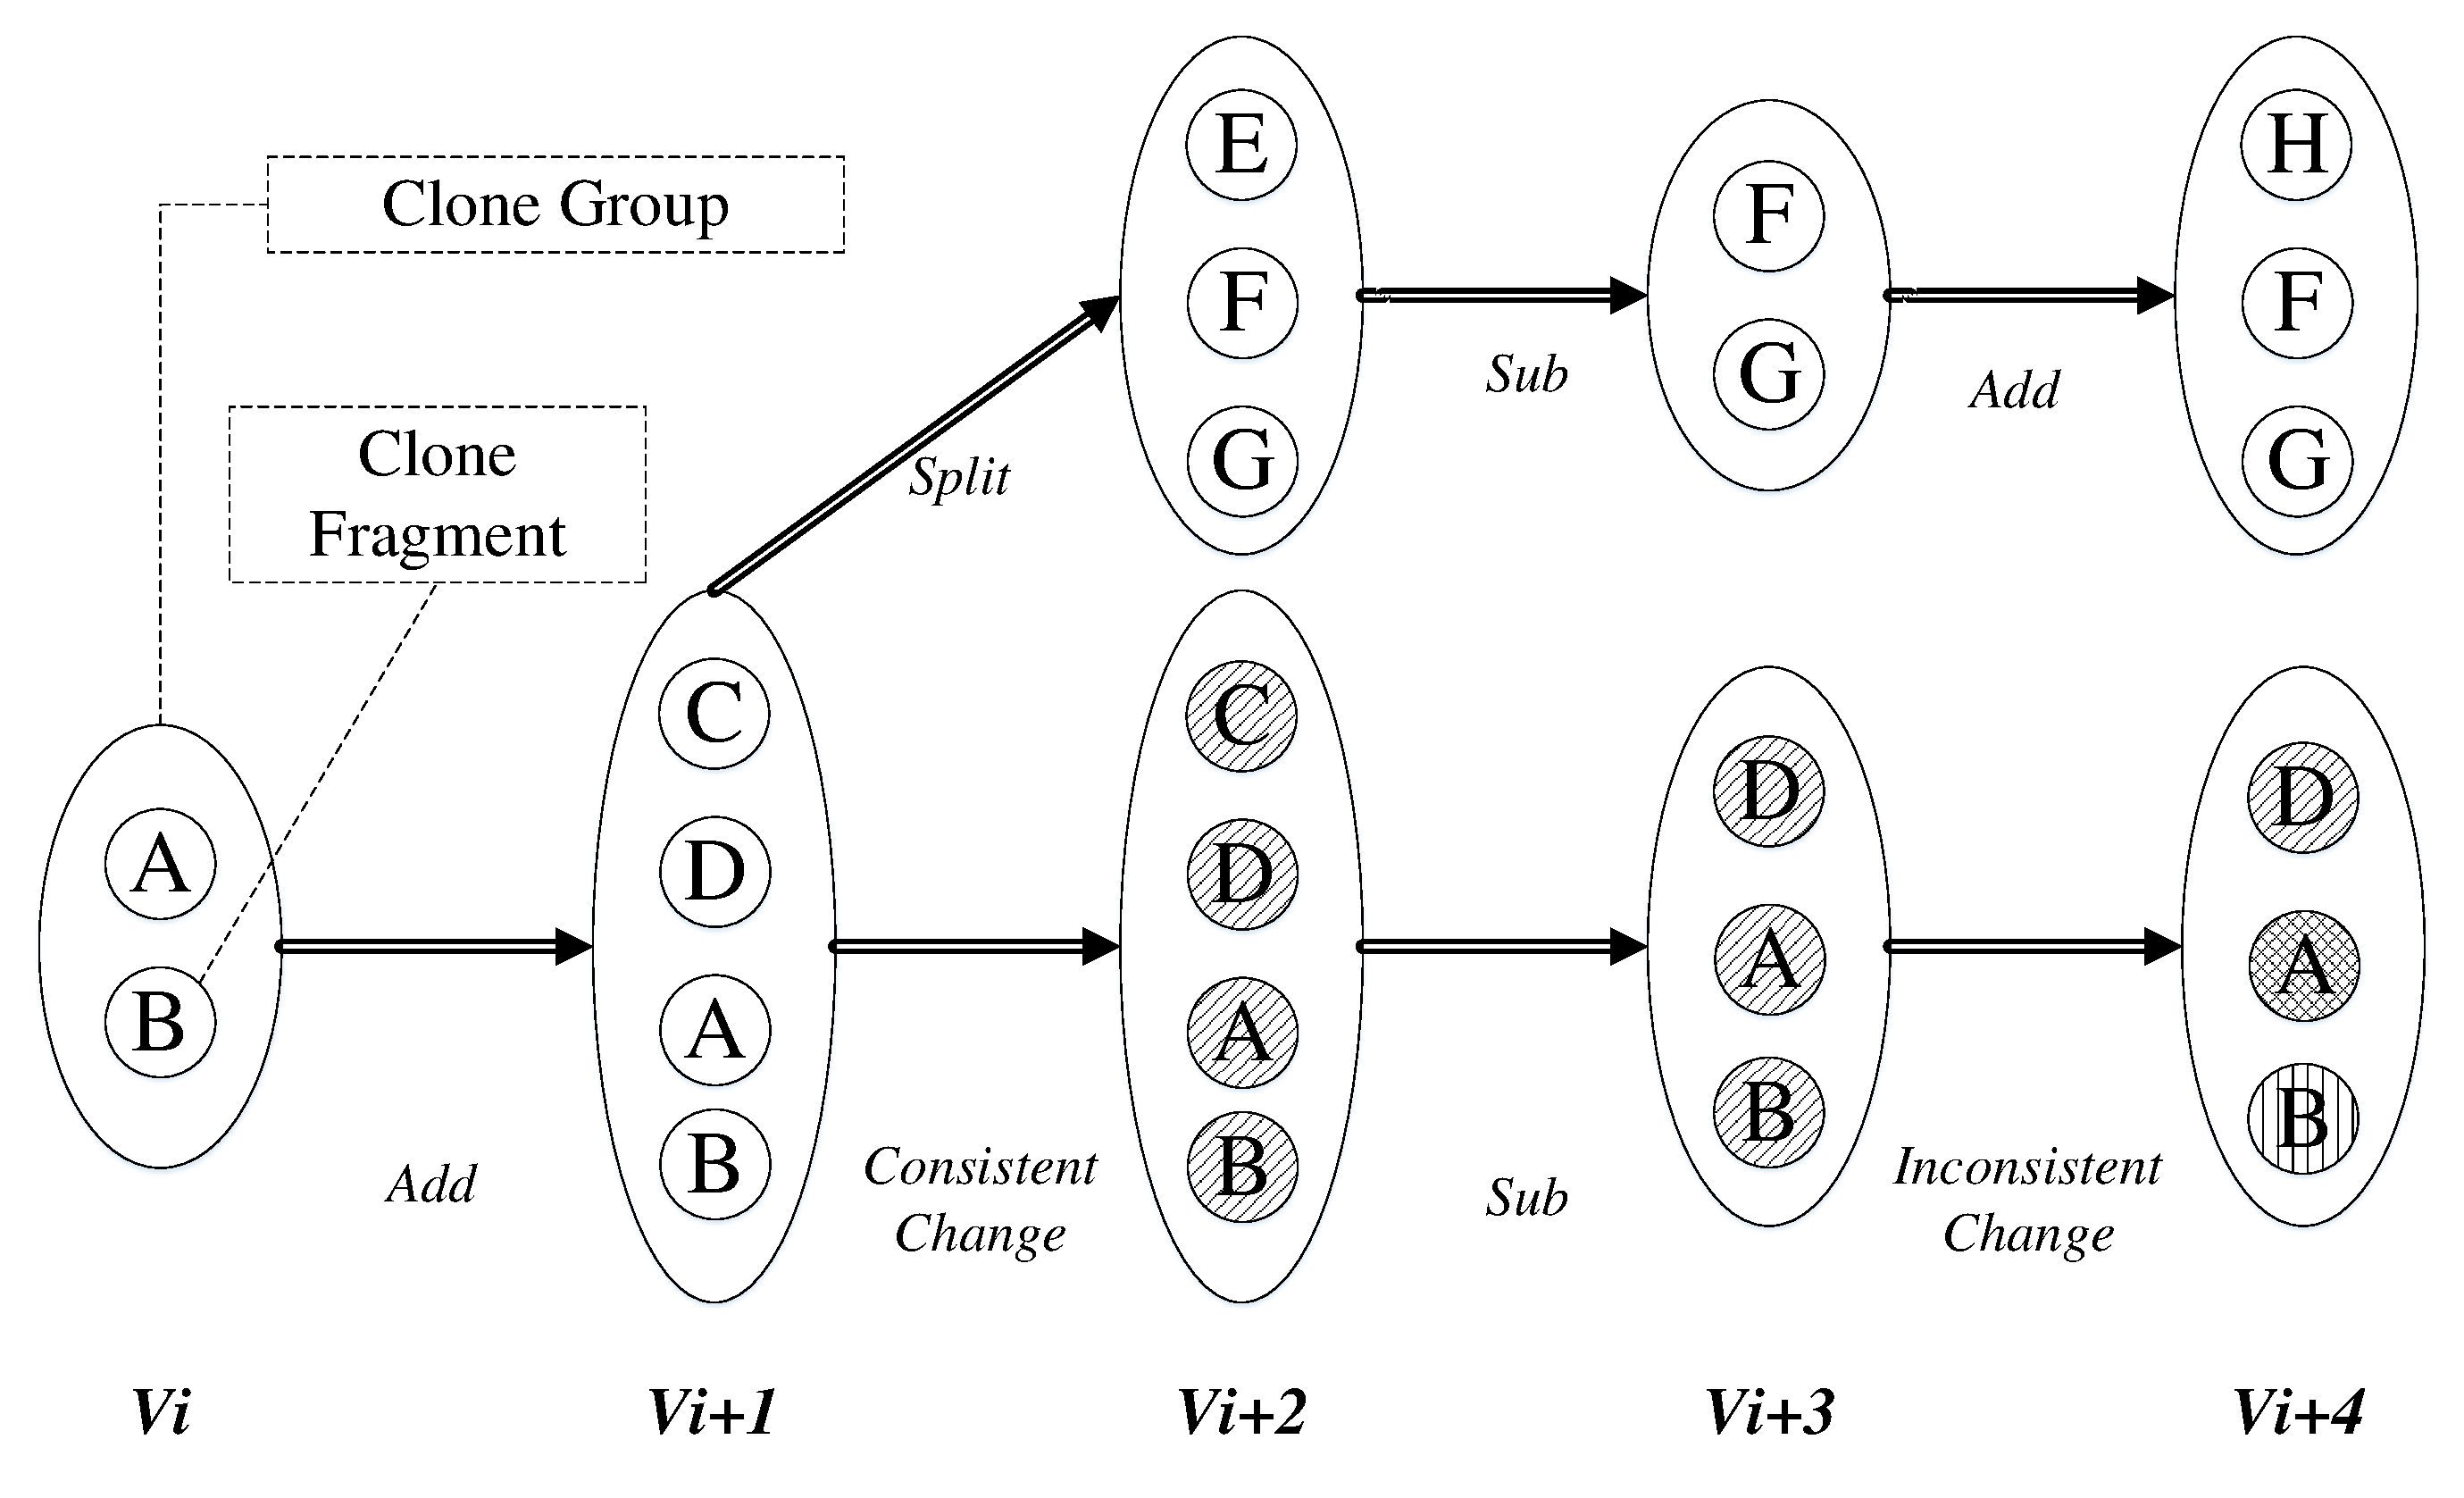
\includegraphics [width=0.7 \textwidth ]{genealogy.pdf}
\bicaption [genealogy]{}{克隆家系示意图}
{Fig.$\!$}{An Example for Clone Genealogy}
\vspace{-1em}
\end{figure}

如图\ref{genealogy}中所示,在克隆组的演化过程中,两个相邻版本间的克隆代码可能会被程序开发人员修改而发生变化,因而也会导致克隆组也会发生变化。在克隆组演化过程中,研究人员使用克隆演化模式描述相邻版本之间的克隆组的变化情况。本文给出7种不同的克隆演化模式,如下所示:

%\begin{definition} [{克隆组演化模式}]
%\label {defn-cge7}
%\item 
%{静态模式 (Static Pattern)}:
%静态模式表示在两个连续版本的演化中该克隆组是静止的,未发生任何变化,即克隆组内的克隆片段数量和内容均未发生变化。
%\item 
%{相同模式(Same Pattern)}:
%相同模式表示在两个连续版本的演化中该克隆组内克隆片段数量无变化,但克隆片段本身可能发生变化。
%\item 
%{增加模式(Add Pattern)}:
%增加模式表示在两个连续版本的演化中该克隆组内的克隆片段数量增加。
%\item 
%{减少模式(Subtract Pattern)}:
%减少模式表示在两个连续版本的演化中该克隆组内的克隆片段数量减少。
%\item 
%{ 一致性变化模式(Consistent Change Pattern)}: 
%一致性变化模式表示在两个连续版本的演化中该克隆组内的克隆片段发生了一致地变化,并且发生变化的克隆片段仍然存在同一克隆组内。
%\item 
%{不一致性变化模式(Inconsistent Change Pattern)}:
%不一致性变化模式表示在两个连续版本的演化中该克隆组内的克隆片段发生了不一致地变化,并且发生变化的克隆片段仍然存在同一克隆组内。
%\item 
{分裂模式(Split Pattern)}:分裂模式表示连续的在两个连续版本的演化中克隆组内克隆片段发生剧烈变化,导致该克隆组分裂成为两个不同的克隆组。
%\end{definition}

\begin{itemize}
\item 
{静态模式 (Static Pattern)}:
静态模式表示在两个连续版本的演化中该克隆组是静止的,未发生任何变化,即克隆组内的克隆片段数量和内容均未发生变化。
\item 
{相同模式(Same Pattern)}:
相同模式表示在两个连续版本的演化中该克隆组内克隆片段数量无变化,但克隆片段本身可能发生变化。
\item 
{增加模式(Add Pattern)}:
增加模式表示在两个连续版本的演化中该克隆组内的克隆片段数量增加。
\item 
{减少模式(Subtract Pattern)}:
减少模式表示在两个连续版本的演化中该克隆组内的克隆片段数量减少。
\item 
{ 一致性变化模式(Consistent Change Pattern)}: 
一致性变化模式表示在两个连续版本的演化中该克隆组内的克隆片段发生了一致地变化,并且发生变化的克隆片段仍然存在同一克隆组内。
\item 
{不一致性变化模式(Inconsistent Change Pattern)}:
不一致性变化模式表示在两个连续版本的演化中该克隆组内的克隆片段发生了不一致地变化,并且发生变化的克隆片段仍然存在同一克隆组内。
\item 
{分裂模式(Split Pattern)}:分裂模式表示连续的在两个连续版本的演化中克隆组内克隆片段发生剧烈变化,导致该克隆组分裂成为两个不同的克隆组。
\end{itemize}

回归到图~\ref{genealogy}中,可以看出在五个版本内该克隆组的演化模式分布情况。从版本{$V_i$}到{$V_i+1$},克隆组新增加了两个克隆片段,因此与之其关联的克隆模式是{Add}。从{ $V_i+1$}到{ $V_i+2$}中,克隆组首先分裂为两组,因此其演化模式为{Split},同时下方的克隆组发生了一致地变化,演化模式为{ Consistent Change}。从版本{$V_i+2$}到{$V_i+3$}中,演化模式一个是{Subtract},另一个是{Inconsistent Change}。 从版本{$V_i+2$}到{$V_i+3$},克隆模式分别是{Add}和{Subtract}。

\BiSubsection{克隆演化特征}
{Clone Evolutionary Characteristics}

克隆家系的提出引发了人们对于克隆代码演化以及演化模式的研究热潮,进而也导致了大量的分析克隆演化特征的研究。克隆演化特征可描述如下:

\begin{definition} [{克隆演化特征}]
\label{defn-characteristics}
{
克隆演化特征指的是克隆代码在演化过程中表现出来的演化特征以及对软件所产生的影响。克隆演化特征不仅可以帮助软件开发人员理解系统中存在的克隆代码,还可以向软件开发人员提供一些如何维护克隆代码的建议。
 }
\end {definition}

究竟哪些演化特征能真实准确地反映克隆代码的规律?这是克隆演化特征分析的难点问题。目前,常用的克隆演化特征主要包括克隆寿命、克隆稳定性与一致性变化(具体如表~\ref{characteristic}所示)。

克隆寿命是指克隆代码在系统中的存在时间,即生存期。Kim研究发现克隆代码要比非克隆代码更加稳定,同时寿命也更长\cite{kim2005empirical};进一步对长寿命的克隆代码进行研究后,发现对克隆代码的修改会使得克隆代码的寿命变短\cite{cai2011empirical}。Krinke通过对比克隆和非克隆代码,也发现克隆代码比非克隆代码的寿命更长\cite{krinke2011cloned}。通过对精确克隆和近似克隆的演化分析,发现其在演化过程中所表现出来的共同特点是:尽管克隆代码比率会随着时间而逐渐降低,但克隆代码的存在时间往往都会超过一年\cite{bazrafshan2012evolution}。因此,克隆代码会长时间的存在于系统中,在其生存期间克隆代码往往会发生变化,其变化规律与具体的软件系统相关\cite{gode2009evolution}。

相对于克隆寿命而言,克隆稳定性关注的是在克隆代码的生存期内是发生变化的问题。被研究者普遍认可的观点是寿命较长的克隆代码是稳定的\cite{krinke2008cloned}\cite{gode2011clone}\cite{harder2013cloned},不会对系统造成不利的影响,也不会增加系统的维护成本。但是在克隆代码是否比非克隆代码更稳定这个问题上还存在一定的分歧。例如Gode研究发现大部分克隆是稳定的,不会发生变化\cite{gode2011frequency}。而Rahman的研究却发现克隆代码比非克隆代码更容易发生变化,是不稳定的\cite{rahman2014change}。Mondal给出了更为细致的分析结果,即Type 1、Type 2克隆是不稳定的,Type 3克隆是稳定的;并且发现克隆代码比非克隆代码的变化更分散,Type 3克隆比Type 1和Type 2克隆的变化更分散\cite{mondal2012comparative}\cite{mondal2012dispersion}。由此可见,在克隆代码的稳定性特征方面尚未达成共识,仍需要进一步研究。

克隆代码的变化包括一致性变化和不一致性变化。开发人员遗忘一致性变化将会引发相关的软件缺陷,如标识符重命名不一致性缺陷等,因此一致性变化也是克隆演化分析研究中需要关注的特征。 Gode的研究发现发生一致性变化的克隆代码占克隆代码的比例很小\cite{gode2011frequency}。Krinke的研究进一步发现发生一致性变化和不一致性变化的克隆代码比例大约各占一半,并且大部分发生不一致性变化的克隆代码在后续的演化过程中不会继续发生变化\cite{krinke2007study}。Mondal等人的研究发现发生一致性变化的克隆代码可能会导致延迟传播现象。延迟传播是指某一个克隆片段的变化没有立即传播到其所在的克隆组中,而在间隔一定数量的版本后传播,继续发生一致性变化。研究表明延迟传播在Type 3的克隆中出现的更为频繁,软件开发人员应该重点关注Type 3克隆代码的变化,以避免引入克隆代码相关的软件缺陷\cite{mondal2016comparative}。

克隆演化特征之间并不是相互独立的,例如克隆寿命会受到稳定性和克隆变化的影响,同时克隆稳定性与克隆变化之间存在对立关系。但是目前的研究中并没有揭示这些关系。更为重要的是,在目前的克隆代码的演化研究中,研究人员的研究往往集中到某一个具体的克隆代码的演化特征上,缺少从宏观上的对克隆代码演化特征的分析。其次,克隆演化研究也往往带有较强的主观性,研究人员往往是通过分析既有的系统验证固有的结论,甚至出现了完全不同的研究结论。因此,如何从大量的克隆代码及其演化过程中全面且客观地识别克隆代码的演化特征是一个值得研究的问题。克隆代码的演化特征对于帮助程序开发人员理解克隆代码及其演化过程具有积极的意义,可以进一步提高软件的可理解性。

\BiSection{基于聚类的克隆代码演化特征分析框架}
{The Framework for Clone Characteristic Analysis based on Clustering}

为分析克隆代码及其演化过程,本文基于机器学习方法提出了一种探索和分析克隆代码演化特征的方法。克隆代码作为具体的代码片段,直接分析其演化过程和特征极为困难。因此,本文将克隆代码及其演化过程抽象成为一些特征向量,并借助机器学习中的聚类方法挖掘克隆代码及其演化过程之间的信息。为了更为具体的抽表示克隆代码及其演化过程,本文用三种不同的克隆实体描述克隆代码及其演化过程,即克隆片段、克隆组和克隆家系实体。在基础上提取相应的度量值表示克隆实体的有意义和有价值信息。最后使用机器学习中的聚类方法分析克隆代码,进而挖掘克隆代码的演化特征。

%WEKA( “Waikato Environment for Knowledge Analysis” \cite{hall2009weka})中实现的X-means\cite{pelleg2000x}方法聚类所有的克隆实体。
%在两个软件系统上进行了实证研究,实证研究结果表明了本文方法可以分析克隆代码的演化特征,可以帮助程序人员理解和维护克隆代码。具体来讲,克隆代在其演化过程中是较为稳定的,在其演化的初始阶段不容易发生变化。程序开打人员因此应该需要更多的关注那些在系统中存在了一定时间的克隆代码(寿命较长的克隆代码)。同时,当克隆代码发生变化的时候,我们也建议尽可能的考虑一致性变化。
%本文的创新点如下:
%\begin{itemize}
%\item 
%本文提出了一个框架分析克隆代码的演化特征,可以帮助程序维护人员维护和管理克隆代码。
%\item 
%本文从三个不同的角度视为将克隆代码一种数据进行分析:克隆片段、克隆组和克隆家系,并提取了相应的度量值表示克隆代码。
%\item 
%本文在两个开源系统上进行了实证研究并获得了相关的克隆演化特征,可以帮助理解和维护克隆代码。
%\end{itemize}

本文所提出的基于聚类的克隆代码演化特征分析框架如图~\ref{framework2}所示。从图中可以看出,本文方法可以划分为三个阶段,分别是预处理阶段、克隆表示阶段和演化特征挖掘阶段。 在预处理阶段,首先检测系统所有版本中的克隆代码,并通过映射连续软件版本之间的克隆代码片以及克隆组来构建系统所有的克隆家系。使用克隆家系可以细致的描述克隆代码的演化过程,同时也可以快速有效的识别克隆代码的演化模式。 在克隆表示阶段阶段,使用三种不同的克隆实体表示克隆代码及其演化过程,并分别提取与之相应的度量值描述不同的克隆实体(克隆片段、克隆组和克隆家系)。所提取的度量值包含了有价值的与克隆代码演化和变化情况的信息。 最后,在演化特征挖掘阶段,使用机器学习方法中的聚类方法来聚类克隆实体向量,并根据聚类结果挖掘克隆代码的克隆演化特征。

\begin{figure}[htbp]
\centering
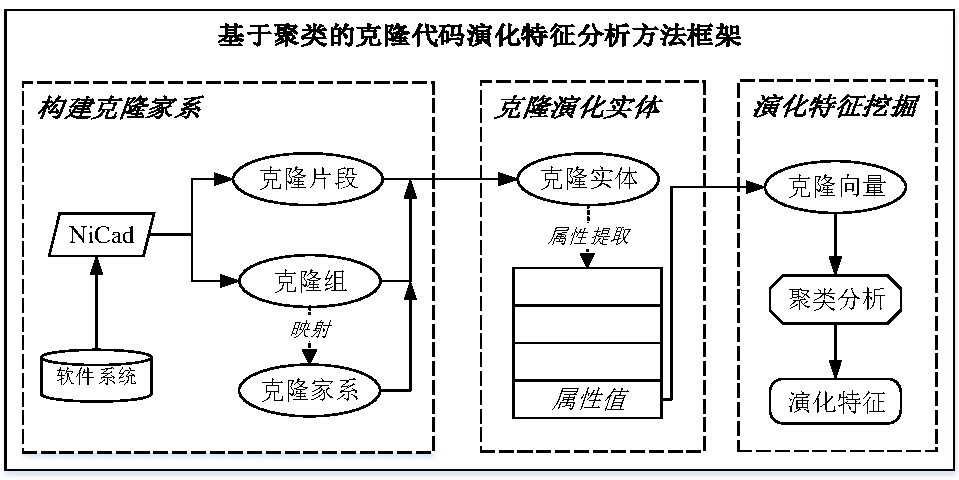
\includegraphics [width=0.9 \textwidth ]{framework2.pdf}
\bicaption [framework2]{}{基于聚类的克隆演化特征提取方法框架}
{Fig.$\!$}{The framework for clone characteristic analysis based on clustering}
%{Fig.$\!$}{The Framework of Clone Characteristic Analysis}
\vspace{-1em}
\end{figure}

值得注意的是,本文方法将克隆代码及其演化过程当做一种数据,然后借助机器学习领域中的聚类分析方法挖掘隐含的信息。在使用聚类分析的时候,由于克隆代码是具体的代码片段,无法直接对其聚类。因此,使用克隆聚类向量表示相应的克隆实体,而克隆聚类向量则是根据克隆实体相应的度量值生成,克隆实体的度量值用于表示克隆代码及其演化过程。本文从三种不同克隆实体表示克隆代码,即克隆片段、克隆组和克隆家系。克隆片段实体是微观角度,从克隆代码自身角度出发,将从克隆代码片段本身是否被修改的角度分析克隆代码的演化特征,所提取的度量值重点关注克隆代码是否被修改。克隆组实体是代码区域角度,从克隆组的角度分析克隆代码演化模式与演化时间的关系, 将揭示克隆组在随着软件演化时所表现出来的特征。克隆家系实体是宏观角度,描述了一个系统中所有的克隆代码(即全部克隆家系)的演化过程以及演化特征。

本文所所采用的聚类分析方法为{\em X-Means}\cite{pelleg2000x}聚类,其原因在于:克隆实体所应聚类的数量具有不确定性,难以确定具体的聚类数量。如果采用人为给定的方式给出聚类的数量,则可能会引入不客观因素,对影响克隆代码演化特征的分析工作。因此,本文采用\em{ X-Means}聚类方法,不需要人为的指定聚类数量,\em{ X-Means}方法会自动地给出最佳的聚类数量。

\BiSection{预处理阶段}
{ Pre-processing Step}

在预处理阶段,将使用克隆检测工具所检测的连续版本软件中的所有克隆代码,并通过映射相邻版本的克隆代码构建系统的克隆家系。首先从开源库中下载连续版本软件的所有源代码,然后使用克隆检测工具NiCad检测克隆代码,最后通过映射克隆代码构建克隆家系和识别克隆演化模式。

\BiSubsection{克隆检测与结果描述}
{Clone Detection and Results’ Representation}

使用克隆检测工具NiCad分别检测系统所有版本中的克隆代码,并使用克隆区域描述符(Clone Region Description, CRD)描述克隆代码位置信息。

为了检测系统中的克隆代码,本文使用{\em NiCad}\cite{roy2008nicad}检测系统中的克隆代码。NiCad是基于文本的克隆检测工具,在工具中集成了程序转换、代码规范化和语法分析技术\cite{cordy2006txl}\cite{dean2003agile},能够以较高的准确度和召回率系统中的Type-1、Type-2和Type-3克隆代码\footnote{NiCad可以从此网站获取:http://www.txl.ca/nicaddownload.html。}。NiCad可以从两个不同粒度检测系统中的克隆代码:函数粒度和块粒度。因为块粒度具有更为通用的检测效果(函数克隆也是是块克隆代码),本文使用{块粒度}检测系克隆代码。根据NiCad的默认配置,其将克隆代码之间的相似度阈值设置为70\%,将相似度高于此阈值的代码片段报告为克隆代码。
%详细介绍相似度

NiCad将检测到的克隆代码保存于XML文件中,并使用\em{ ``Filename + Start/End Line No''}标记克隆克隆代码,并将彼此相似的克隆片段保存在同一克隆组内。由于NiCad仅仅使用代码行表示克隆代码,不仅无法描述克隆代码的语法和语义信息,也不利于映射不同版本之间的克隆代码。因此,为映射相邻版本之间的克隆代码,本文使用改进的克隆区域描述符表示克隆代码,并在此基础上实现克隆代码的映射和克隆家系的构建。克隆区域描述符最早由Duala-Ekoko等人提出,不仅可以反映出克隆代码本身的信息,还可以用于跟踪演化过程中的克隆代码\cite{duala2010clone}。为了进一步的帮助映射相邻版本之间的克隆代码,慈蒙等人改进了克隆区域描述符,并提出了基于克隆区域描述符的克隆群映射算法\cite{ci2013new}。
为了映射两个相邻版本中的克隆代码和克隆组,新添加相对位置覆盖率和文本相似度两个额外的表示单元。使用相对位置覆盖率可以帮助定位源代码中的克隆片段,并计算版本$ i $和版本$ i + 1 $中克隆片段位置之间的重叠率。文本相似度可以用于比较映射的代码片段的相似性度。具体方法可以参加慈蒙等人的论文\cite{ci2013newD}。
%这里使用NiCad中的计算方法。它计算两个克隆片段的常用代码行的百分比。
%%添加详细的算法描述。

\BiSubsection{克隆家系构建与克隆模式识别}
{Building Clone Genealogy and Identifying Representation}

为了映射连续版本的克隆代码,使用基于克隆区域描述符的映射算法,生成所有相邻版本的映射结果,并根据映射结果构建克隆家系和识别克隆演化模式。

构建克隆家系的关键步骤在于映射所有相邻版本间的克隆片段,而相邻版本间的克隆群映射关系则可以根据克隆群内的克隆片段的映射关系进行确定。所采用的映射算法称为基于CRD的克隆代码映射算法\cite{ci2013new}\cite{ci2013newD}。假设给定一个软件系统的两个相邻版本{$V_i$}和{$V_ {i + 1}$},并分别检测两个版本之间的克隆代码,并使用CRD描述所检测到的克隆代码。为了映射两个版本间的克隆代码,将{ $V_i$}中的每个克隆片段与下一版本{$ V_{i+1}$}中的每个克隆片段进行比较,寻找与之映射的克隆片段,并生成克隆片段的映射结果。于此同时,根据克隆片段的映射结果,也可以实现相邻版本中所有克隆组的映射。更进一步,将所有相邻版本之间的克隆代码进行映射,并根据映射结果生成系统中的所有的克隆家系。

克隆演化模式可以用于描述克隆组在演化过程中的变化情况,对于揭示克隆演化特征具有重要的意义。克隆演化模式识别,可以通过对比映射的两个相邻版本之间的克隆组进行。假设克隆组$CG$是存在于相邻的两个软件版本{$(V_i,V_{i+1})$}中,且克隆组$CG$的映射关系可以使用{$(CG_i, CG_{i+1})$}描述,其中{$CG_i$}表示前一版本中的克隆组,{$CG_{i+1}$}表示后一版本中的克隆组。通过观察从{$CG_i$}到{$CG_{i+1}$}的克隆组变化情况,便可以识别该克隆组{$CG$}的克隆演化模式。

\BiSection{克隆表示阶段}
{Clone Representation Step}

为挖掘克隆代码的演化特征,本文将从三个不同角度分析克隆代码及其演化情况,即克隆片段、克隆组和克隆家系,并将之称为克隆代码实体(克隆实体)。正如在机器学习中通常所做的那样,本文还提取不同的度量值表示不同的克隆实体。对克隆片段实体,本文重点关注克隆代码的变化情况。对克隆家系实体,本文重点关注克隆演化模式的情况。对于克隆家系实体,本文重点关注系统所有的克隆演化模式的情况。

\BiSubsection{克隆片段度量}
{Clone Fragment Attributes}

克隆片段度量给出了克隆代码本身的一些特征。在克隆片段的生命期间,克隆片段可能被程序人员开发人员修改(特别是在软件维护期间),即克隆片段在演化过程中可能会发生变化,甚至可能发生不止一次的变化。

因此,本文将克隆代码变化次数(截止到系统当前版本$V_i$)和是否发生了变化(从上一版本演化到此版本时)视为克隆片段的度量,即在某一软件版本$V_ i $中的克隆代码片段{$CF_i$}度量如下所示:
\begin{itemize}
\item
克隆寿命(Clone Life):
截止到当前版本$V_ i $,克隆片段$CF$所经历的所有的版本数量称之为克隆寿命。
%\item {Clone Life}: number of versions which the clone fragment exists in software so far (until version i).
\item
是否发生变化(Ischanged):
从上一版本$V_ {i-1} $演化到此版本$V_ i $时,克隆片段$CF$是否发生了变化,若发生变化则取值为$1$,否则取值为$0$。
%\item {Ischanged}:	equals 1 if the Clone fragment in version i is changed from the last version (version i-1); 0 otherwise.
\item
变化次数(Change Times):
截止到当前版本$V_ i $,克隆片段$CF$在其演化过程中所发生的变化次数。
%\item {Change Times}:	number of times the clone fragment changed so far (up till version i) in the evolution.  
\end{itemize}

\BiSubsection{克隆组度量}
{Clone Group Attributes}

克隆组提供了克隆代码的一些区域性特征。本文所使用的克隆演化模式均是针对克隆组而言,因此也需要从克隆组的角度分析克隆代码的演化情况。对于某一个克隆组,最先提取的度量是克隆寿命。克隆寿命不但揭示了其在系统中存在的时间长短,也与克隆演化模式息息相关。在克隆组进行演化的过程中,克隆模式更是从演化的角度揭示了克隆组的变化情况。因此,本文将版本$V_i $ 中克隆组{$CG_i$}的寿命和克隆演化模式提取为度量值,如下所示:
\begin{itemize}
\item
克隆寿命(Group Life):
截止到当前版本$V_ i $,克隆组$CG$所经历的所有的版本数量称之为克隆寿命。
%\item {Group Life}: number of versions which clone group exists in software till version $i$.
\item
静态(Static):
克隆组$CG$从上一版本$V_ {i_1} $演化到$V_ i $时,是否发生了静态模式(Static Pattern)。
%\item {Static}:	all clone fragments in group are static from last version.
\item
相同(Same):
克隆组$CG$从上一版本$V_ {i_1} $演化到$V_ i $时,是否发生了相同模式(Same Pattern)。
%\item {Same}:	clone group undergoes a ``same'' pattern change from  last version.
\item
增加(Add):
克隆组$CG$从上一版本$V_ {i_1} $演化到$V_ i $时,是否发生了增加模式(Add Pattern)。
%\item {Add}: clone group undergoes an ``add'' pattern change from last version.
\item
减少(Subtract):
克隆组$CG$从上一版本$V_ {i_1} $演化到$V_ i $时,是否发生了减少模式(Subtract Pattern)。
%\item {Subtract}: clone group undergoes a ``subtract'' pattern change from last version.
\item
一致性变化(Consistent Change):
克隆组$CG$从上一版本$V_ {i_1} $演化到$V_ i $时,是否发生了一致性变化模式(Consistent Change Pattern)。
%\item {Consistent Change}: clone group undergoes a ``consistent change'' pattern from last version.
\item
不一致变化(Inconsistent Change):
克隆组$CG$从上一版本$V_ {i_1} $演化到$V_ i $时,是否发生了不一致变化模式(Inconsistent Change Pattern)。
%\item {Inconsistent Change}: clone group undergoes an ``inconsistent change'' pattern from last version.
\item
分裂(Split):
克隆组$CG$从上一版本$V_ {i_1} $演化到$V_ i $时,是否发生了分裂模式(Split Pattern)。
%\item {Split}: clone group undergoes a ``split'' pattern change from last version.
\end{itemize}

\BiSubsection{克隆家系度量}
{Clone Genealogy Attributes}

克隆家系提供了一个软件中克隆代码演化的全局视角,从而可以帮助捕获软件系统整个生命期间的克隆代码的演化特征。如前文所述,一个克隆组{$CG$}在所有的版本中的演化过程即是一个克隆家系{$CGE$},因此一个软件系统中将会有很多个克隆家系。对于每一个克隆家系{$CGE$},本文提取{克隆寿命}和{克隆演化模式数量}作为克隆家系{$CGE$}的度量。{ 克隆寿命}是克隆家系的一个极为重要的指标,描述了克隆代码在系统中存在的时间。同时,克隆家系还描述了一个克隆组在整个生命期间的全部演化过程(所经历的克隆演化模式数量)。演化模式数量揭示了克隆组的整个变化历史。因此某一克隆家系{$CGE$}的属性如下所示:

\begin{itemize}
\item
克隆家系寿命(Genealogy  Life):
克隆家系{$CGE$}在其整个演化过程中所经历的软件版本的数量。
%\item Genealogy  Life: number of versions which clone genealogy exists in software.
\item
静态模式数量(Static Number):
克隆家系{$CGE$}在其整个演化过程中所经历的静态模式的数量。
%\item Static Number: number of ``static'' pattern which all clone groups belonging to this genealogy have experienced in its life.
\item
相同模式数量(Same Number):
克隆家系{$CGE$}在其整个演化过程中所经历的相同模式的数量。
%\item Same Number: number of ``same'' pattern which all clone groups belonging to this genealogy have experienced in its life.
\item
增加模式数量(Add Number):
克隆家系{$CGE$}在其整个演化过程中所经历的增加模式的数量。
%\item Add Number: number of ``add'' pattern which all clone groups belonging to this genealogy have experienced  in its life.
\item
减少模式数量(Subtract Number):
克隆家系{$CGE$}在其整个演化过程中所经历的减少模式的数量。
%\item Subtract Number: number of ``subtract'' pattern which all clone groups belonging to this genealogy have experienced in its life.
\item
一致性变化模式数量(Consistent Number):
克隆家系{$CGE$}在其整个演化过程中所经历的一致性变化模式的数量。
%\item Consistent Number: number of ``consistent pattern'' which all clone groups belonging to this genealogy have experienced in its life.
\item
不一致变化模式数量(Inconsistent Number):
克隆家系{$CGE$}在其整个演化过程中所经历的不一致变化模式的数量。
%\item Inconsistent Number: number of ``inconsistent pattern'' which all clone groups belonging to this clone genealogy have experienced in its life.
\item
分裂模式数量(Split Number):
克隆家系{$CGE$}在其整个演化过程中所经历的分裂模式的数量。
%\item Split Number: number of ``split'' pattern which all clone groups belonging to this genealogy have experienced in its life.
\end{itemize}

\BiSection{演化特征挖掘阶段}
{Evolutionary Characteristics Mining Step}

为了从克隆代码及其演化过程中挖掘演化特征,本文将使用使用WEKA( “Waikato Environment for Knowledge Analysis” \cite{hall2009weka})中提供的聚类方法来分析克隆代码,将从克隆片段、克隆组和克隆家系三个不同的角度进行分聚类析。本文将这个挖掘任务分成两个子任务:第一,对获得的所有克隆实体进行统计分析,并且根据统计分析结果获取克隆代码的演化特征。第二,使用WEKA对克隆实体进行聚类分析,根据聚类结果获取克隆代码的演化特征。%在这个子任务中,主要目标是分析在软件演化过程中克隆代码的寿命以及变化情况,即确定克隆变化在克隆演化中所发生的时间以及变化。为此,我们在WEKA中使用工具来对包含时间元素的克隆实体进行聚类。在这个子任务中,


\BiSubsection{克隆实体聚类}
{Clone Entity Clustering}

使用WEKA聚类克隆实体也可以划分为三个部分:首先,为每一个克隆实体成一个“克隆聚类向量”,包含每个克隆实体的所有度量值。然后,使用克隆聚类向量生成克隆聚类空间,表示不同的克隆实体。最后,使用WEKA聚类这些克隆向量,并根据聚类结果提取克隆代码演化特征。

 首先,为每一个克隆实体生成克隆聚类向量。 对于每个克隆片段、克隆组和克隆家系实体,其聚类向量是一个$m$维向量:即{$Vector$ ={($v_1$,$v_2$,$...$,$v_m$)}},其中$v_i$表示该克隆实体的一个特定度量值。以某一克隆组{$CG$}为例,为该克隆组{$CG$}生成一个8维向量{$Vector$ =($v_1$,$v_2$,$...$,$v_8$)},其中$v_i$(对于所有$i$ , $i \leq $ 8)是此克隆组{$CG$}对应的度量值。
 
然后,生成所有克隆代码实体的聚类向量空间。为了聚类所有的克隆实体,本文将生成系统的全部克隆聚类向量。所有克隆实体的聚类向量可以组成聚类向量空间$X$。$X$可以由{$X$={($x_1$,$x_2$,$...$,$x_n$)}}表示,其中$n$是克隆实体的数量。本文从克隆片段、克隆组和克隆家系三个角度考聚类分析克隆代码,因此也有三个不同的克隆向量空间:$X_{CF}$、$X_{CG}$和$X_{CGE}$,其中$X_{CF}$表示所有的克隆片段聚类空间,$X_{CG}$表示所有的克隆组聚类空间,$X_{CGE}$表示所有的克隆家系聚类空间。
  
最后,使用WEKA聚类克隆特征向量。WEKA是一个用于数据挖掘的流行机器学习工具,WEKA中实现了许多方法来分析数据,例如聚类,分类,关联规则等等(本文所使用的聚类方法由WEKA实现)\footnote{WEKA是新西兰怀卡托大学用Java开发的数据挖掘软件工具,其几乎可以运行在所有操作系统平台上。其网站是:http://www.cs.waikato.ac.nz/ml/weka/}。 克隆代码的向量空间$X_{CF}$、$X_{CG}$和$X_{CGE}$分别表示了系统中全部的克隆片段、克隆组和克隆家系。本文使用聚类方法聚类这三个不同的向量空间,并分析得到克隆演化特征。

\BiSubsection{X-means聚类}
{X-means Clustering}

本文选择的聚类方法是X-means聚类\cite{pelleg2000x}, X-means聚类是K-means聚类\cite{arthur2007k}的改进方法。后者可以将$X$向量空间聚类为事前指定的$K$个Cluster中,并使得相似的向量分配到同一个Cluster中。但是,K-means聚类必须制定所需要聚类的Cluster的数量。然而对于克隆代码聚类而言,难以确定所需的Cluster的数目,因此本文选择使用X-means聚类。X-means聚类并不需要具体的指定Cluster数量,其会自动搜索最佳的Cluster数量,因此更为适合于克隆代码演化特征的聚类分析。

X-means聚类是一种高效的聚类算法,可以通过自动搜索并确定聚类数量\cite{pelleg2000x}。给定一个克隆向量空间$X$ = {($x_1$,$x_2$,$...$,$x_n$)},其中每个$x_i$是$d$维实向量)。X-means聚类将向量空间$X$ 中的$n$个向量划分为$k$个Clusters,即 $C$ = {($C_1$,$C_2$,$...$,$C_k$)},$C_i$表示一个Cluster。使用X-means聚类只需要指定$K$的范围即可,聚类算法会自动的搜索最佳的Cluster数量$K$。
%过程如下:算法从给定的$K$范围的最低值开始,并继续增加此值,直到范围的上限。在此过程中,X-means聚类使用模型选择标准计算每个$K$的分数。它选择$K$的最高分数输出。对于每个$K$,x-means聚类使用迭代细化技术。首先,它将每个向量分配给其平均值产生集群内最小平方和(WCSS)的集群。第二,它计算新的均值为新聚类中的向量的质心。当分配不再改变时,算法收敛。它使用后验概率用贝叶斯信息准则对这$j$进行评分。

\BiSection{实验结果与分析}
{The Results and Discussion}
\label{ref-characteristics}
\BiSubsection{实验设置}
{Experiment Methodology}

在本节中,首先简要描述了所使用的开源实验系统,并描述了从三个不同克隆视角挖掘克隆演化特征的实验步骤。

选择两个开源软件作为本章的实验系统:分别为{ArgoUML}和{ jEdit},两个开源系统都至少经历了10个版本的演化。%\em{ ArgoUML}是一个领先的开源UML建模工具,包括对所有标准UML 1.4图的支持。\em{ jEdit}是另一个开源项目,是程序员开发所使用的编辑器,其特点是具有易于使用的接口,类似于许多流行的文本编辑器。都是使用Java语言开发的软件
表~\ref{statisticsofcluster}描述了这两个实验系统的基本信息。从表中第2-4列可以看出,{ArgoUML}经历了$14 $个版本的演化(起始和结束版本分别为$0.20.0$和$0.34.0$),{ jEdit}经历了$22$个版本的演化(起始和结束版本分别为$3.0.0$和$5.0.0$)。表中第5-6列则给出了实验系统的克隆实体数量(克隆聚类空间大小)。其中,“Clone Fragment”列出了所聚类的克隆片段的数量,“Clone Group”和“Clone Genealogy”分别是所聚类的克隆组和克隆家系数量。

\begin{table}[htbp]
\bicaption [statisticsofcluster]{}{两个开源软件实验系统信息}
{Table$\!$}{The information of two open sources experimental projects }
%{Table$\!$}{The Two Open Sources Experiments Software for }
\vspace{0.5em}
\centering 
\wuhao
\begin{tabular}{ccccccc}
\toprule[1.5pt ]
\multirow{2}{*}{Projects}&\multirow{2}{*}{Versions}&Start&End&Clone&Clone&Clone\\ 
&&Version&Version&Fragment&Group&Genealogy\\
\midrule[1pt]
ArgoUML&14&0.20.0&0.34.0&25422&7012&1036\\ 
jEdit&22&3.0.0&5.0.0&6636&2256	&237\\ 
\bottomrule[1.5pt]
\end{tabular}
\end{table}

本章实验可以分为三个部分,从克隆片段、克隆组和克隆家系三个不同的视角挖掘和分析克隆代码的演化特征,即克隆片段实验、克隆组实验和克隆家系实验。在克隆片段实验中,重点分析克隆片段在演化过程中的变化情况。 在克隆组实验中,分析克隆组在演化过程中的克隆演化模式情况,并重点分析了克隆代码的一致性和不一致变化模式。在克隆家系的实验中,从全局的角度分析了系统中全部克隆代码的演化规律,重点讨论了克隆代码的稳定性以及一致性变化问题。

在每个实验中,本文均使用两种方法分析和挖掘克隆代码的演化特征:统计分析和聚类分析。第一种统计分析每种克隆实体的度量值,进而发现一些基本的演化特征。第二种是聚类分析方法,使用{X-means}分别聚类每一种克隆实体,并根据聚类结果深入挖掘克隆代码的演化特征。

\BiSubsection{克隆片段实验}
{Clone Fragment Experiment}

克隆片段是指软件中存在的真实的代码片段, 在其生命周期内,克隆片段可能会被开发人员修改。克隆片段实验中考虑克隆片段的三个度量值,分别是{\em Clone Life、Ischanged、Change Times},上述度量值将帮助了解克隆片段在其演化过程中的真实变化情况。

首先,对克隆片段变化次数进行了统计分析,分析结果如表~\ref{cfstaargouml}~和表~\ref{cfstajedit}~所示。从表中可以看出,大多数克隆片段在演化过程中并不会发生变化(未发生变化的克隆片段数量在{ArgoUML}中为$24327$个,在{\em  jEdit}中为$5885$)。同时 只有仅仅一小部分克隆片段在演化过程中发生了变化({ArgoUML}为$1095$个,{jEdit}为$751$个)。值得注意的是,在发生变化的克隆片段中有极少数的克隆片段被改变了不止一次,其数量随着改变次数的增大而减少。 因此可以得出结论:{克隆片段在其生命期间是十分稳定的(大多数克隆片段从未发生变化),但依然存在一定数量的克隆代码片段发生了变化;且在发生变化的克隆片段中,克隆变化不会频繁地发生,仅有极少量的克隆代码会频繁的发生变化。}

\begin{table}[htbp]
\bicaption[cfstaargouml]{}{ArgoUML中克隆片段的变化情况统计}
{Table$\!$}{The statistic of clone fragment change for ArgoUML}
%{Table$\!$}{Clone Fragment  Change Statistic of ArgoUML}
\vspace{0.5em}
\centering
\wuhao
\begin{tabular}{ccccc}
\toprule[1.5pt]
Change Times&0&1&2&3\\ 
\midrule[1pt]
Number&24327&982&109&4\\ 
Total&24327&\multicolumn{3}{c}{1095} \\
\bottomrule[1.5pt]
\end{tabular}
\end{table}

\begin{table}[htbp]
\bicaption[cfstajedit]{}{jEdit中克隆片段的变化情况统计}
{Table$\!$}{The statistic of clone fragment change for jEdit}
%{Table$\!$}{Clone Fragment Change Statistic of jEdit}
\vspace{0.5em}
\centering
\wuhao
\begin{tabular}{ccccccccc}
\toprule[1.5pt]
Change Times &0&1&2&3&4&5&6&7\\ 
\midrule[1pt]
Number&5885&533&135&47&14&10&11&1\\ 
Total&5885&\multicolumn{7}{c}{751}   \\ 
\bottomrule[1.5pt]
\end{tabular}
\end{table}

随后,使用X-means方法对克隆片段进行聚类分析,实验结果如表~\ref{cfcluargouml}~和~\ref{cfclujedit}~所示。X-means聚类将{ArgoUML}和{jEdit}的克隆代码片段分成4个Cluster:即Cluster0--Cluster4。本文根据聚类结果分别统计了四个Cluster的度量值信息,即平均值(Mean)、标准差(Standard Deviation,SD)和中位数(Median)。从表中可以看出,在{ArgoUML}和{jEdit}两个开源软件中,Cluster0的克隆片段中数量最少,该Cluster中的克隆代码在其演化的过程中发生过变化(Change Times约等于1),本文将这些克隆片段称为{changed}克隆片段。因此,{在所有的克隆代码片段中仅有少量的克隆代码片段发生过变化,同时相对于未发生变化的克隆代码(Cluster3,ischanged和Change Times均为0),发生变化的时刻往往是其存在于系统中一段时间后(对比Clone Life}。除此之外,根据``{isChanged}''列可以看出,在系统{ArgoUML}中的Cluster1、Cluster3和系统{jEdit}中的Cluster1、Cluster2和Cluster3中,所有的克隆片段都没有发生变化,它们的数量占到克隆片段数量的多数。这意味着{大多数的克隆片段在其演化的过程中是稳定的,不会发生变化}。最后,系统{ArgoUML}和{jEdit}中的Cluster3是完全没有发生变化的克隆片段,根据其寿命发现它们在软件中存在的时间极短 。这表明{刚刚出现在系统中的克隆是极其稳定的(在短时间内不会发生变化)}。因此,我程序开发人员应该更多地关注{那些已经存在系统中一段时间(存在几个版本)的克隆代码片段,因为它们更容易发生变化。}


\begin{table}[htbp]
\bicaption[cfcluargouml]{}{ArgoUML中克隆片段的聚类结果}
{Table$\!$}{Clustering results of clone fragment for ArgoUML}
\vspace{0.5em}
\centering
\footnotesize
%\wuhao
\begin{tabular}{ccccccccccc}
\toprule[1.5pt]
\multirow{2}{*}{Cluster}&{Number}&\multicolumn{3}{c}{Clone Life}&\multicolumn{3}{c}{Ischanged}&\multicolumn{3}{c}{Change Times} \\
&(Percentage)&{Mean}&SD &{Median}&{Mean}&SD &{Median}&{Mean}&SD &{Median}\\
%\multirow{3}{*}{Cluster}&{Number}&\multicolumn{3}{c}{Clone Life}&\multicolumn{3}{c}{Ischanged}&\multicolumn{3}{c}{Change Times} \\
%&(Percentage)&\multirow{2}{*}{Mean}& Standard &\multirow{2}{*}{Median}&\multirow{2}{*}{Mean}&Standard &\multirow{2}{*}{Median}&\multirow{2}{*}{Mean}&Standard &\multirow{2}{*}{Median}\\
%&&&  Deviation&&& Deviation&&& Deviation&\\ 
\midrule[1pt]
Cluster 0&899(4\%)&7.207&2.299&7&0.092&0.290&0&1.130&0.350&1\\ 
Cluster 1&3082(12\%)&7.763&1.523&8&0&0&0	&0&0&0\\ 
Cluster 2&3006(12\%)&3.833&0.871&4&0.058&0.234&0	&0.065&0.247&0\\ 
Cluster 3&18435(73\%)&1.094&0.292&1	&0	&0	&0	&0	&0	&0\\ 
\bottomrule[1.5pt]
\end{tabular}
\end{table}

\begin{table}[htbp]
\bicaption[cfclujedit]{}{jEdit中克隆片段的聚类结果}
{Table$\!$}{Clustering results of clone fragment for jEdit}
\vspace{0.5em}
\centering
\footnotesize
%\wuhao
\begin{tabular}{ccccccccccc}
\toprule[1.5pt]
\multirow{2}{*}{Cluster}&{Number}&\multicolumn{3}{c}{Clone Life}&\multicolumn{3}{c}{Ischanged}&\multicolumn{3}{c}{Change Times} \\
&(Percentage)&{Mean}&SD &{Median}&{Mean}&SD&{Median}&{Mean}&SD &{Median}\\
%\multirow{3}{*}{Cluster}&{Number}&\multicolumn{3}{c}{Clone Life}&\multicolumn{3}{c}{Ischanged}&\multicolumn{3}{c}{Change Times} \\
%&(Percentage)&\multirow{2}{*}{Mean}& Standard &\multirow{2}{*}{Median}&\multirow{2}{*}{Mean}&Standard &\multirow{2}{*}{Median}&\multirow{2}{*}{Mean}&Standard &\multirow{2}{*}{Median}\\
%&&&  Deviation&&& Deviation&&& Deviation&\\ 
\midrule[1pt]
Cluster 0&200(3\%)&5.325&2.690&5&1	&0	&1	&1.64	&1.148&1\\ 
Cluster 1&1371(21\%)	&9.071&2.885&8	&0	&0	&0	&0.503&0.916&0\\ 
Cluster 2&	1624(15\%)	&4.227&1.112&4	&0	&0	&0	&0.065&0.261&0\\ 
Cluster 3&	3441(66\%)	&1.175	&0.3780&1	&0	&0	&0	&0	&0	&0\\ 
\bottomrule[1.5pt]
\end{tabular}
\end{table}

%%\begin{table}[htbp]
%%\bicaption[cfcluargouml]{}{ArgoUML中克隆片段的聚类结果}
%%{Table$\!$}{Clone Fragment Clustering Results of ArgoUML}
%%\vspace{0.5em}
%%\centering
%%\wuhao
%%\begin{tabular}{ccccccccccc}
%%\toprule[1.5pt]
%%\multirow{2}{*}{Cluster}&{Number}&\multicolumn{3}{c}{Clone Life}&%%\multicolumn{3}{c}{Ischanged}&\multicolumn{3}{c}{Change Times} \\
%%&(Percentage)&{Mean}&SD &{Median}&{Mean}&SD &{Median}&{Mean}&SD %%&{Median}\\
%%%%%\multirow{3}{*}{Cluster}&{Number}&\multicolumn{3}{c}{Clone Life}&\multicolumn{3}{c}{Ischanged}&\multicolumn{3}{c}{Change Times} \\
%%%%%%%&(Percentage)&\multirow{2}{*}{Mean}& Standard &\multirow{2}{*}{Median}&\multirow{2}{*}{Mean}&Standard &\multirow{2}{*}{Median}&\multirow{2}{*}{Mean}&Standard &\multirow{2}{*}{Median}\\
%%%%%&&&  Deviation&&& Deviation&&& Deviation&\\ 
%%\midrule[1pt]
%%Cluster 0&899(4\%)&7.2069&2.2993&7&0.09232&0.28965&0&1.13014&0.34963&1\\ 
%%Cluster 1&3082(12\%)&7.76314&1.52307&8&0&0&0	&0&0&0\\ 
%%Cluster 2&3006(12\%)&3.833&0.8707&4&0.05822&0.23419	&0	&0.0652&0.24692&0\\ 
%%Cluster 3&18435(73\%)&1.09401&0.29184	&1	&0	&0	&0	&0	&0	&0\\ 
%%\bottomrule[1.5pt]
%%\end{tabular}
%%\end{table}

%%\begin{table}[htbp]
%%\bicaption[cfclujedit]{}{jEdit中克隆片段的聚类结果}
%%{Table$\!$}{Clone Fragment Clustering Results of jEdit}
%%\vspace{0.5em}
%%\centering
%%\wuhao
%%\begin{tabular}{ccccccccccc}
%%\toprule[1.5pt]
%%\multirow{2}{*}{Cluster}&{Number}&\multicolumn{3}{c}{Clone Life}&\multicolumn{3}{c}{Ischanged}&\multicolumn{3}{c}{Change Times} \\
%%&(Percentage)&{Mean}&SD &{Median}&{Mean}&SD&{Median}&{Mean}&SD &{Median}\\
%%%%%\multirow{3}{*}{Cluster}&{Number}&\multicolumn{3}{c}{Clone Life}&\multicolumn{3}{c}{Ischanged}&\multicolumn{3}{c}{Change Times} \\
%%%%%&(Percentage)&\multirow{2}{*}{Mean}& Standard &\multirow{2}{*}{Median}&\multirow{2}{*}{Mean}&Standard &\multirow{2}{*}{Median}&\multirow{2}{*}{Mean}&Standard &\multirow{2}{*}{Median}\\
%%%%%&&&  Deviation&&& Deviation&&& Deviation&\\ 
%%\midrule[1pt]
%%Cluster 0&	200(3\%)	&5.325	&2.6899	&5	&1	&0	&1	&1.64	&1.1476	&1\\ 
%%Cluster 1&	1371(21\%)	&9.07075	&2.88542	&8	&0	&0	&0	&0.50328	&0.91649	&0\\ 
%%Cluster 2&	1624(15\%)	&4.2266	&1.11192	&4	&0	&0	&0	&0.06466	&0.26059	&0\\ 
%%Cluster 3&	3441(66\%)	&1.17495	&0.37998	&1	&0	&0	&0	&0	&0	&0\\ 
%%\bottomrule[1.5pt]
%%\end{tabular}
%%\end{table}

综上所述,只有少数的克隆代码片段在软件演化过程中会发生变化,同时这些克隆片段所经历的变化通常发生在它们在系统中存在一段时间之后。

\BiSubsection{克隆组实验}
{Clone Group Experiment} 

{克隆片段}实验仅提供了克隆片段本身的变化情况,而通过对{克隆组}进行实验分析则可以提供了克隆代码以克隆组为单位的克隆变化情况。 在克隆组实验中,通过统计和聚类克隆组在演化过程中的克隆演化模式,从而揭示克隆代码的演化特征。

本文首先统计了克隆组的{“克隆演化模式”(Clone Pattern)}数量,结果如表~\ref{cgstaargouml}~和~\ref{cgstajedit}~所示。表中使用“Present”和“Absent”来标识克隆组是否具有某种具体克隆演化模式\footnote{克隆组的演化模式之间不是相互独立的,一个克隆组可以具有多个演化模式,例如可以同时具有“Static”和“Same”。}。同时,本文也非正式地将克隆演化模式中“Static”模式和“Same”模式称为“稳定的克隆演化模式”(Stable Clone Pattern),其它的克隆模式称为“动态的克隆模式”(Dynamic Clone Pattern)。从表中可看出,在两个实验系统中,大多数的克隆组(比例约72\% - 85\%)具有有稳定的克隆模式,只有一小部分克隆组(其比例小于7\%)具有动态的克隆模式(即具有Add,Sustract,Split,Consistent/Inconsistent Change)。值得注意的是,在ArgoUML和jEdit中有数百个克隆组具有Consistent/Inconsistent Change模式。这应该引起程序开发人员的注意,因为这种变化模式-- 特别是Consistent Change模式-- 会导致额外的维护代价甚至会引发相关的克隆缺陷。从表中可以看出,在系统jEdit和ArgoUML中,发生一致变化(Consistent Change)模式的克隆组要多于不一致变化(Inconsistent Change)模式的克隆组(ArgoUM具有两种模式克隆组数量分别为:$350$和$329$,jEdit为$140$和$41$)。因此可以得出结论:相比于不一致变化模式,软件系统中的克隆组更容易发生一致性的变化。
%本文首先统计了克隆组的{“克隆演化模式”(Clone Pattern)}数量,结果如表~\ref{cgstaargouml}~和~\ref{cgstajedit}~所示。表中使用“Present”和“Absent”来标识克隆组是否具有某种具体克隆演化模式\footnote{克隆组的演化模式之间不是相互独立的,一个克隆组可以具有多个演化模式,例如可以同时具有“Static”和“Same”。}。同时,本文也非正式地将克隆演化模式中“静态”模式和“相同”模式称为“稳定的克隆演化模式”(Stable Clone Pattern),其它的克隆模式称为“动态的克隆模式”(Dynamic Clone Pattern)。从表中可看出,在两个实验系统中,大多数的克隆组(比例约72\% - 85\%)具有有稳定的克隆模式,只有一小部分克隆组(其比例小于7\%)具有动态的克隆模式(即具有Add,Sustract,Split,Consistent/Inconsistent Change)。值得注意的是,在ArgoUML和jEdit中有数百个克隆组具有一致性/不一致变化模式。这应该引起程序开发人员的注意,因为这种变化模式-- 特别是一致性变化-- 会导致额外的维护代价甚至会引发相关的克隆缺陷。从表中可以看出,在系统jEdit和ArgoUML中,发生一致变化模式的克隆组要多于不一致变化模式的克隆组(ArgoUM具有两种模式克隆组数量分别为:$350$和$329$,jEdit为$140$和$41$)。因此可以得出结论:相比于不一致变化模式,软件系统中的克隆组更容易发生一致性的变化。

\begin{table}[htbp]
\bicaption[cgstaargouml]{}{ArgoUML中克隆组的演化模式统计}
{Table$\!$}{The statistic of clone group evolution pattern for ArgoUML}
\vspace{0.5em}
\centering
%\footnotesize
\wuhao
\begin{tabular}{cccccccc}
\toprule[1.5pt]
Number of&\multirow{2}{*}{Static}&\multirow{2}{*}{Same}&\multirow{2}{*}{Add}&\multirow{2}{*}{Subtract}&Consistent&Inconsistent&\multirow{2}{*}{Split}\\ 
Groups&&&&&Change&Change&\\ 
\midrule[1pt]
Present	&5114	&5422	&345	&324	&350	&329	&36\\ 
Absent	&1898	&1590	&6667	&6688	&6662	&6683	&6976\\ 
Percentage	&72.93\%	&77.40\%	&4.92\%	&4.62\%	&5.25\%	&4.69\%	&0.51\%\\ 
\bottomrule[1.5pt]
\end{tabular}
\end{table}

\begin{table}[htbp]
\bicaption[cgstajedit]{}{jEdit中克隆组的演化模式统计}
{Table$\!$}{The statistic of clone group evolution pattern for jEdit}
\vspace{0.5em}
\centering
%\footnotesize
\wuhao
\begin{tabular}{cccccccc}
\toprule[1.5pt]
Number of&\multirow{2}{*}{Static}&\multirow{2}{*}{Same}&\multirow{2}{*}{Add}&\multirow{2}{*}{Subtract}&Consistent&Inconsistent&\multirow{2}{*}{Split}\\ 
Groups&&&&&Change&Change&\\ 
\midrule[1pt]
Present	&1783	&1922	&45	&36	&140	&41	&19\\ 
Absent	&473	&334	&2211	&2220	&2116	&2215	&2237\\ 
Percentage	&79.3\%	&85.20\%	&1.99\%	&1.60\%	&6.21\%	&1.82\%	&0.84\%\\ 
\bottomrule[1.5pt]
\end{tabular}
\end{table}

表~\ref{cgcluargouml}~和~\ref{cgclujedit}~给出了克隆组聚类分析的结果。与克隆片段聚类实验相似,聚类结果也分成了四类。本文统计了每一类的克隆组的演化模式,并使用“Mean”表示平均值、“SD”表示标准差、“Median”表示中位数。从表中可以看出,Cluster1的克隆组的数量最多(在ArgoUML中比例为71\%,在jEdit中占79\%)。Cluster1的克隆组比较稳定(克隆组具有稳定的克隆模式,并且没有动态的克隆模式),同时具有相对较长的寿命。因此,大多数的克隆组是非常稳定的,也具有相对较长的寿命(在两个软件中大约5个版本)。同时,从表中还可以看出大多数的{不一致变化模式(Inconsistent Change Pattern)}出现在Cluster0中,并且仅仅占用很小的比例(ArgoUML中的4\%,在jEdit中只有1\%)。因此可以得出结论不一致变化模式在克隆组中不会频繁发生。另外,一致性变化模式(Consistent Change Pattern)仅发生在Cluster2中,其存在的克隆组的寿命相对较长,但相比于Cluster0会短一些。值得注意的是,Cluster0和Cluster2都是动态克隆组,因为这些克隆组都具有动态的克隆演化模式。因此得出结论,动态的克隆演化模式往往会发生在较为长寿的克隆组中,但是它们的数量非常小。

从Cluster0 和Cluster2中克隆组的绝对数量上看,具有一致性变化模式的克隆组(Cluster2)的数量大于具有不一致变化模式的克隆组数量(Cluster0)。这意味着一致性变化模式相比于不一致性变化模式更容易发生。因此本文建议:开发人员在修改克隆组中某一克隆片段时需要考虑同时修改组内其它的克隆片段,即考虑克隆代码的一致性变化问题。

同时从Cluster3中可以看出,有相当一部分的克隆组具有极短的寿命(刚刚出现在系统中),因此其并没有相关的克隆演化模式。这也意味着在克隆组刚刚创建的初始版本中并不不需要考虑克隆组的变化情况以及对系统的影响问题。


\begin{table}[htbp]
\bicaption[cgcluargouml]{}{ArgoUML中克隆组的聚类结果}
{Table$\!$}{Clustering results of clone group for ArgoUML}
\vspace{0.5em}
\centering
\footnotesize
%\wuhao
\begin{tabular}{cccccccccc}
\toprule[1.5pt]
\multirow{2}{*}{Cluster}&\multirow{2}{*}{Metric}&Group&Static &Same &Add &Subtract &Consistent &	Inconsistent &Split \\ 
&&Life& Number& Number& Number& Number& Number&	 Number& Number\\ 
\midrule[1pt]
Cluster0&Mean&	3.042	&0.587	&0.701	&1	&1	&0	&1	&0.080\\ 
264&SD&2.251	&0.493	&0.459	&0	&0	&0	&0	&0.271\\ 
(4\%)&Median	&2	&1	&1	&1  &1	&0	&1	&0\\ 
\hline
Cluster1&Mean	&4.909&1	&1	&0	&0	&0	&4.03E-4	&6.05E-4\\ 
4959&SD&3.098&0	&0	&0	&0	&0	&0.020&0.025\\ 
(71\%)&Median	&5	&1	&1	&0	&0	&0	&0	&0\\ 
\hline
Cluster2&Mean	&3.389&0	&0.670&0.186&0.145&0.843	&0.152&0.019\\ 
415&SD&2.666&0	&0.471&0.389&0.352&0.364	&0.360&0.138\\ 
(6\%)&Median	&2	&0	&1	&0	&0	&1	&0	&0\\ 
\hline
Cluster3&Mean	&0.608&0	&0	&0.003&0	&0	&0	&0.003\\ 
1374&SD&0.520&0	&0	&0.054&0	&0	&0	&0.054\\ 
(20\%)&Median	&1	&0	&0	&0	&0	&0	&0	&0\\
\bottomrule[1.5pt]
\end{tabular}
\end{table}

\begin{table}[htbp]
\bicaption[cgclujedit]{}{jEdit中克隆组的聚类结果}
{Table$\!$}{Clustering results of clone group for jEdit}
\vspace{0.5em}
\centering
\footnotesize
%\wuhao
\begin{tabular}{cccccccccc}
\toprule[1.5pt]
\multirow{2}{*}{Cluster}&\multirow{2}{*}{Metric}&Group&Static &Same &Add &Subtract &Consistent &	Inconsistent &Split \\ 
&&Life& Number& Number& Number& Number& Number&	 Number& Number\\ 
\midrule[1pt]
Cluster0&	Mean	&6.88	&0.4	&0.76	&1	&1	&0	&1	&0.2\\
25	&SD&4.438	&0.5	&0.436	&0	&0	&0	&0	&0.408\\ 
(1\%)	&Median	&7	&0	&1	&1	&1	&0	&1	&0\\ 
\hline
Cluster1	&Mean	&5.762	&1	&1	&0	&0	&0	&0	&5.64E-4\\
1773	&SD&4.05197	&0	&0	&0	&0	&0	&0	&0.024\\
(79\%)&	Median&	5	&1&	1&	0&	0&	0&	0&	0\\ 
\hline\
Cluster2	&Mean	&5.362&	0&	0.872&	0.128&	0&	0.94&	0.027&	0.060\\
149&	SD&	3.780&	0&	0.335&	0.335&	0&	0.239 &	0.162 &	0.239 \\ 
(7\%)&	Median&	4&	0&	1&	0&	0&	1&	0&	0\\ 
\hline
Cluster3	&Mean	&0.997&	0&	0	&0.003&0.036	&0	&0.039	&0.013\\ 
309	&SD&1.239&0	&0	&0.057&0.186&0	&0.194&0.113\\ 
(14\%)&	Median&	1&	0&	0&	0&	0&	0&	0&	0\\ 
\bottomrule[1.5pt]
\end{tabular}
\end{table}


%%\begin{table}[htbp]
%%\bicaption[cgcluargouml]{}{ArgoUML中克隆组的聚类结果}
%%{Table$\!$}{Clone Group Clustering Results of ArgoUML}
%%\vspace{0.5em}
%%\centering\wuhao
%%\begin{tabular}{cccccccccc}
%%\toprule[1.5pt]
%% \multirow{2}{*}&\multirow{2}{*}&Group&Static &Same &Add &Subtract &Consistent &	Inconsistent &Split \\ 
%%&&Life& Number& Number& Number& Number& Number&	 Number& Number\\ 
%%\midrule[1pt]
%%Cluster0&Mean&	3.04167	&0.58712	&0.70076	&1	&1	&0	&1	&0.07955\\ \cline{2-10}
%%264&Standard Deviation	&2.25093	&0.49329	&0.4588	&0	&0	&0	&0	&0.2711\\ \cline{2-10}
%%(4\%)&Median	&2	&1	&1	&1  &1	&0	&1	&0\\ \hline
%%Cluster1&Mean	&4.90926	&1	&1	&0	&0	&0	&4.03307E-4	&6.04961E-4\\ \cline{2-10}
%%4959&Standard Deviation	&3.0984	&0	&0	&0	&0	&0	&0.02008	&0.02459\\ \cline{2-10}
%%(71\%)&Median	&5	&1	&1	&0	&0	&0	&0	&0\\ \hline
%%Cluster2&Mean	&3.38795	&0	&0.66988	&0.18554	&0.14458	&0.84337	&0.15181	&0.01928\\ \cline{2-10}
%%415&Standard Deviation	&2.66601	&0	&0.47082	&0.38921	&0.3521	&0.36389	&0.35927	&0.13766\\ \cline{2-10}
%%(6\%)&Median	&2	&0	&1	&0	&0	&1	&0	&0\\ \hline
%%Cluster3&Mean	&0.60844	&0	&0	&0.00291	&0	&0	&0	&0.00291\\ \cline{2-10}
%%1374&Standard Deviation	&0.52006	&0	&0	&0.0539	&0	&0	&0	&0.0539\\ \cline{2-10}
%%(20\%)&Median	&1	&0	&0	&0	&0	&0	&0	&0\\
%%\bottomrule[1.5pt]
%%\end{tabular}
%%\end{table}

%%\begin{table}[htbp]
%%\bicaption[cgclujedit]{}{jEdit中克隆组的聚类结果}
%%{Table$\!$}{Clone Group Clustering Results of jEdit}
%%\vspace{0.5em}
%%\centering\wuhao
%%\begin{tabular}{cccccccccc}
%%\toprule[1.5pt]
%%\multicolumn{10}{c}{\bf Table 9.\  Clone Group Clustering Results of jEdit }\\ 
%% \multirow{2}{*}&\multirow{2}{*}&Group&Static &Same &Add &Subtract &Consistent &	Inconsistent &Split \\ 
%%&&Life& Number& Number& Number& Number& Number&	 Number& Number\\ 
%%\midrule[1pt]
%%Cluster0&	Mean	&6.88	&0.4	&0.76	&1	&1	&0	&1	&0.2\\ \cline{2-10}
%%25	&Standard Deviation	&4.43772	&0.5	&0.43589	&0	&0	&0	&0	&0.40825\\ %%\cline{2-10}
%%(1\%)	&Median	&7	&0	&1	&1	&1	&0	&1	&0\\ \hline
%%Cluster1	&Mean	&5.76199	&1	&1	&0	&0	&0	&0	&5.64016E-4\\ \cline{2-10}
%%1773	&Standard Deviation	&4.05197	&0	&0	&0	&0	&0	&0	&0.02375\\ \cline{2-10}
%%(79\%)&	Median&	5	&1&	1&	0&	0&	0&	0&	0\\ \hline\
%%Cluster2	&Mean	&5.36242&	0&	0.87248&	0.12752&	0&	0.9396&	0.02685&	0.0604\\\cline{2-10}
%%149&	Standard Deviation&	3.77977&	0&	0.33468&	0.33468&	0&	0.23903&	0.16218&	0.23903\\ 
%%\cline{2-10}
%%(7\%)&	Median&	4&	0&	1&	0&	0&	1&	0&	0\\ \hline
%%Cluster3	&Mean	&0.99676&	0&	0	&0.00324	&0.0356	&0	&0.03883	&0.01294\\ \cline{2-10}
%%309	&Standard Deviation	&1.23924	&0	&0	&0.05689	&0.18559	&0	&0.19351	&0.11322\\ \cline{2-10}
%%(14\%)&	Median&	1&	0&	0&	0&	0&	0&	0&	0\\ 
%%\bottomrule[1.5pt]
%%\end{tabular}
%%\end{table}

综上所述,克隆组在其演化过程中通常是非常稳定的。当克隆组存在于系统的一段时间之后,动态的克隆演化模式可会发生在一小部分的克隆组中。同时,当开发人员修改某一克隆片段时,本文建议需要考虑克隆组内其它克隆片段是否需要一致性修改,即确定克隆组变化的一致性。

\BiSubsection{克隆家系实验}
{Clone Genealogy Experiment} 

克隆家系可以提供系统中克隆代码的全局视角,因此本文也对克隆家系进行了实验。在克隆家系实验中,本文依然首先统计了克隆家系在其整个生命周期中的克隆演化模式数量,然后使用X-means对克隆家系进行聚类分析,从而挖掘和分析克隆代码的演化特征。
 
\begin{figure}[htbp]
\centering
\subfigure{\label{cgestargo}}
\addtocounter{subfigure}{-2}
\subfigure[The statistics of clone genealogy evolution for ArgoUML]
{\subfigure[ArgoUML中克隆家系的演化模式统计]{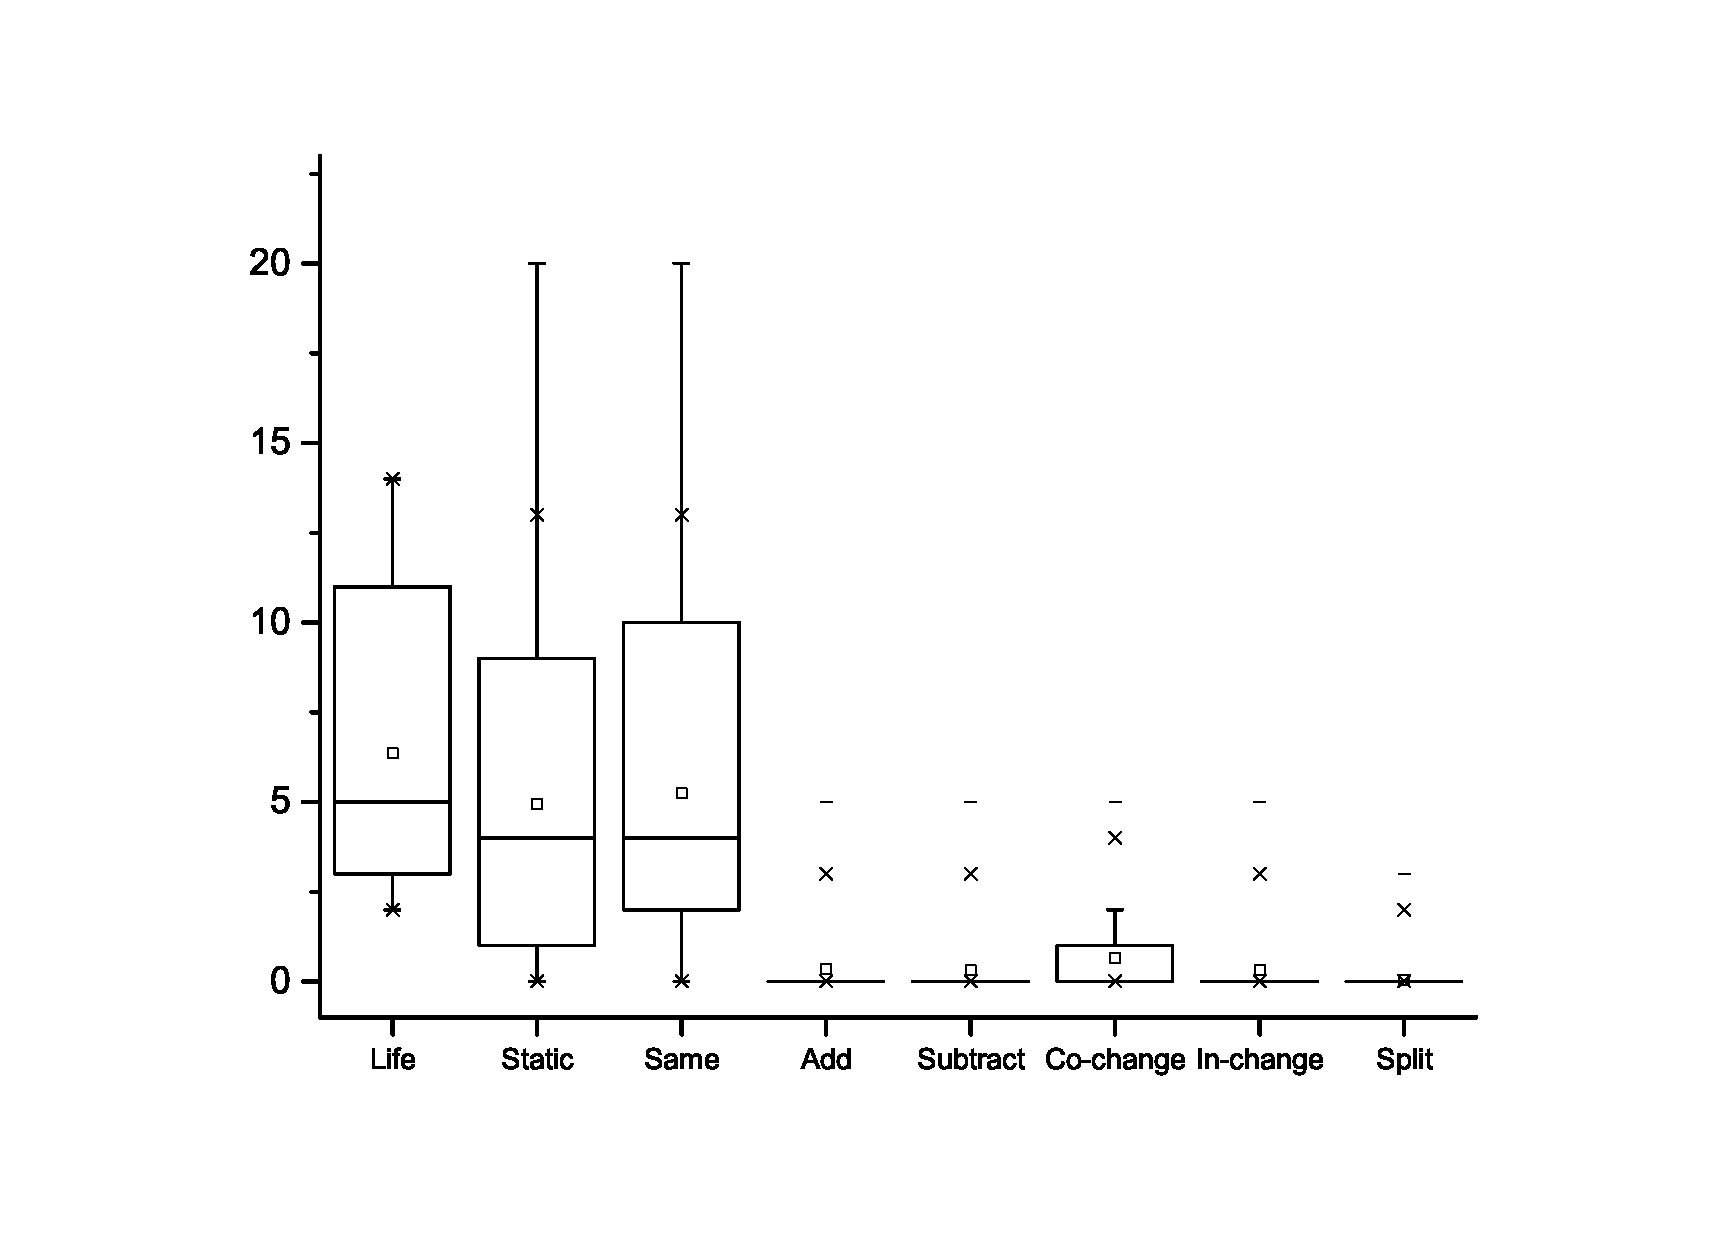
\includegraphics[width=0.8\textwidth]{cgestargo.eps}}}
\subfigure{\label{cgestjedit}}
\addtocounter{subfigure}{-2}
\subfigure[The statistics of clone genealogy evolution for jEdit]
{\subfigure[jEdit中克隆家系的演化模式统计]{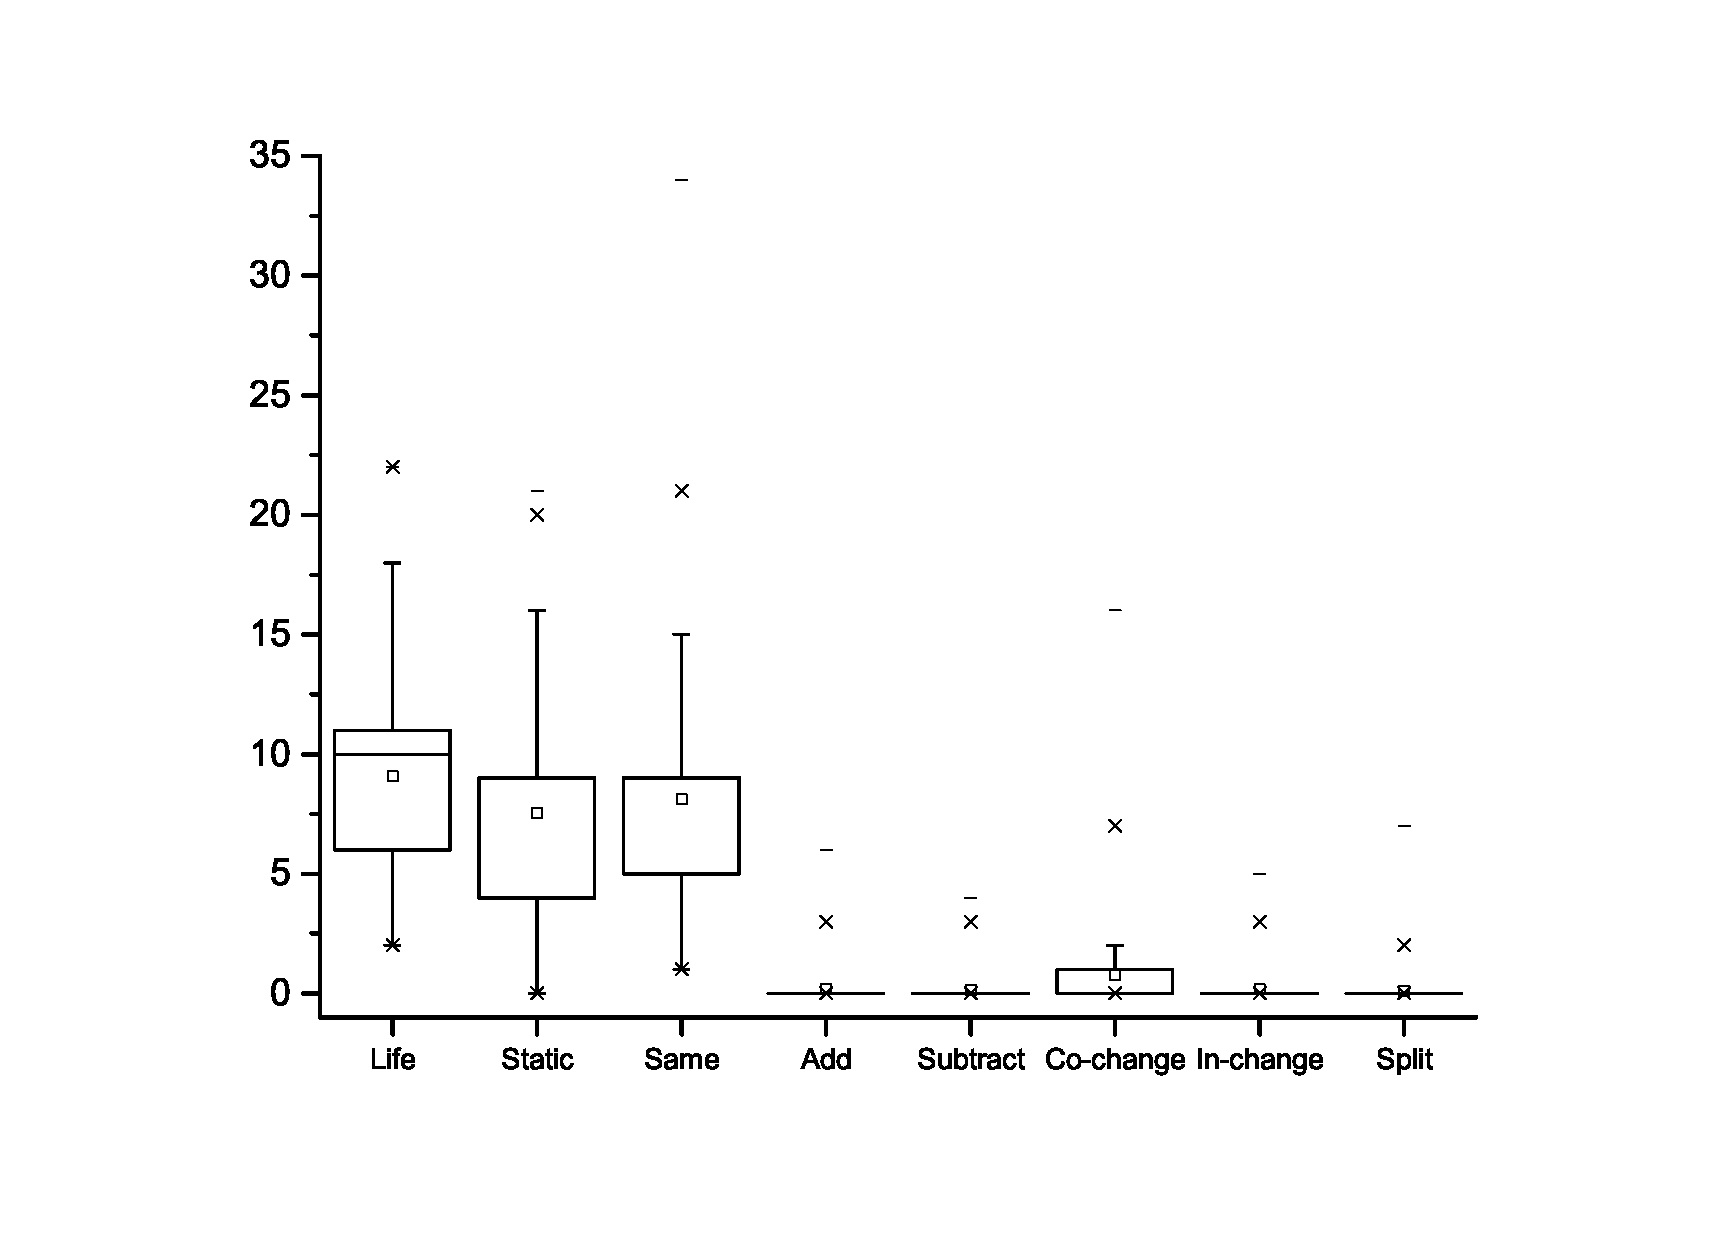
\includegraphics[width=0.8\textwidth]{cgestjedit.eps}}}
\bicaption[cgestas]{}{克隆家系的演化模式统计}
{Fig.$\!$}{The statistics of clone genealogy evolution}
\vspace{-1em}
\end{figure}

本文首先统计了克隆家系的所有度量值(包括克隆寿命和克隆演化模式数量),统计结果如图~\ref{cgestas}~所示。结果使用箱式图展示, 图中横坐标表示克隆家系的演化情况,即本文所选用的克隆家系的度量值,纵坐标表示克隆家系度量值的数值范围。
 
从图中的“Life”可以看出,克隆家系在系统中会存在相当长的一段时间(Clone Life的平均值,ArgoUML中的克隆家系在全部14个版本中存在约5个版本, jEdit的克隆家系在22版本中存在约10个版本)。同时,只有一小部分克隆家系存在极短的时间(少于3个版本)或极长的时间(多于10个版本)。另外,还可以看到 静态的演化模式(Static和Same)的数量要远远高于动态的演化模式的数量。 在动态的演化模式中,一致性变化(图中Co-change)和不一致变化(图中In-Change)模式的数量非常少,这意味着克隆家系在克隆演化的整个生命期间是非常稳定的。具体地,一致性变化模式的数量也多于超过不一致性变化模式的数量。 这也意味着在演化过程中克隆代码更容易发生一致性变化,因此当修改克隆代码时,应该考虑是克隆代码的一致性问题。
 
\begin{table}[htbp]
\bicaption[cgecluargouml]{}{ArgoUML中克隆家系的聚类结果}
{Table$\!$}{Clustering results of clone genealogy for ArgoUML}
\vspace{0.5em}
\centering
\footnotesize
%\wuhao
\begin{tabular}{ccccccccccc}
\toprule[1.5pt]
Cluster&Death&Metric&Life&	Static&	Same&	Add	&Subtract&	Consistent&	Inconsistent&	Split\\ 
\midrule[1pt]
Cluster0&\multirow{3}{*}{5}&Mean	&11.854	&9.795	&10.451	&2.232&	2.232&	3.061&	2.293&	0.390\\ 
82&&SD&1.820&2.989&	3.048&	1.046&	1.081&0.851&1.071&	0.843\\ 
(8\%)&&Median	&11&	10&	10&	2&	2&	3&	2	&0\\ 
\hline
Cluster1&\multirow{3}{*}{39}&Mean	&10.192&8.831&9.096	&0.171&0.122	&0.444&0.122&0.005\\ 
385&&SD&	1.680	&1.676&1.703&0.398&	0.328	&0.648&	0.328	&0.102\\ 
(37\%)&&Median	&11	&9	&10	&0&	0&	0&	0	&0\\ 
\hline
Cluster2&\multirow{3}{*}{188}&Mean	&3.294&1.255	&2	&0.471&0.461&1.260	&0.461	&0.010\\
204&&SD&1.228&1.355&1.324&0.639&0.6389&0.440&0.638&0.140\\ 
(20\%)&&Median	&3&	1&	2&	0&	0&	1&	0&	0\\ 
\hline
Cluster3&\multirow{3}{*}{348}&Mean	&2.795	&1.795	&1.795	&0	&0	&0	&0	&0\\ 
365&&SD&1.081	&1.081&1.081&0	&0	&0	&0	&0\\ 
(35\%)&&Median	&3	&2	&2	&0	&0	&0&	0&	0\\ 
\hline
All&\multirow{3}{*}{579}&Mean	&6.359&4.936&5.234&0.333	&0.313&0.655	&0.318&0.035\\ 
1036&&SD&4.025	&4.022	&4.062	&0.750	&0.745&0.974&0.757&0.272\\ 
(100\%)&&Median&	5&	4&	4&	0&	0&	0&	0&	0\\
\bottomrule[1.5pt]
\end{tabular}
\end{table}

\begin{table}[htbp]
\bicaption[cgeclujedit]{}{jEdit中克隆家系的聚类结果}
{Table$\!$}{Clustering results of clone genealogy for jEdit}
\vspace{0.5em}
\centering
\footnotesize
%\wuhao
\begin{tabular}{ccccccccccc}
\toprule[1.5pt]
Cluster&Death&Metric&Life&	Static&	Same&	Add	&Subtract&	Consistent&	Inconsistent&	Split\\
\midrule[1pt]
Cluster0&\multirow{3}{*}{3}&Mean	&19	&15.8	&19.2	&3	&2.3&	6	&2.7&	1.1\\ 
10&&SD&4.830&4.566&	6.426&1.333&	0.949&	4.570&	1.418&2.234\\ 
(4\%)&&Median	&22&	17&	19&	3&	2	&4.5	&2.5&	0\\ 
\hline
Cluster1&\multirow{3}{*}{35}&Mean	&10.952&	9.445&	9.938&	0.075	&0.075	&0.589&	0.082&	0.041\\ 
146&&SD&2.356&2.166&2.358&0.265	&0.313&	1.074&	0.343&	0.285\\ 
(62\%)&&Median&	10&	9&	9	&0&	0	&0	&0&	0\\ 
\hline
Cluster2&\multirow{3}{*}{24}&Mean	&6.571&	4.75&	5.607&	0.071&	0.071&	0.857&	0.071&	0.071\\ 
28&&SD&1.168&	1.143&1.227&0.262&0.262&0.970&0.262&0.378\\ 
(12\%)&&Median	&7	&5	&6&	0	&0	&1&	0&	0\\ \hline
Cluster3&\multirow{3}{*}{48}&Mean	&3.340&	2.132&	2.302&	0.038&	0	&0.208&	0	&0\\ 
53&&SD&	0.732&0.921&0.723&	0.192&	0&	0.454&0	&0\\ 
(22\%)&&Median	&3&	2&	2	&0&	0&	0	&0&	0\\ \hline
All&\multirow{3}{*}{110}&Mean	&9.072&7.523&	8.110&0.190&	0.152&	0.764	&0.173&	0.080\\ 
237&&SD&4.366&	4.079&4.569&0.690&	0.554&	1.706&0.664	&0.550\\ 
(100\%)&&Median	&10	&9	&9	&0	&0	&0	&0	&0\\
\bottomrule[1.5pt]
\end{tabular}
\end{table}

 
%%%begin{table}[htbp]
%%%\bicaption[cggcluargouml]{}{ArgoUML中克隆家系的聚类结果}
%%%{Table$\!$}{Clone Genealogy Clustering Results of ArgoUML}
%%%\vspace{0.5em}
%%%\centering\wuhao
%%%\begin{tabular}{ccccccccccc}
%%%\toprule[1.5pt]
%%% &Death&&Genealogy Life&	Static&	Same&	Add	&Subtract&	Consistent&	Inconsistent&	Split\\ 
%%%\midrule[1pt]
%%%Cluster0&\multirow{3}{*}{5}&Mean	&11.85366	&9.79268	&10.45122	&2.23171&	2.23171&	3.06098&	2.29268&	0.39024\\ \cline{3-11}
%%%82&&Standard Deviation	&1.81979	&2.98861&	3.04758&	1.04585&	1.08068	&0.85125&1.07138&	0.84263\\ \cline{3-11}
%%%(8\%)&&Median	&11&	10&	10&	2&	2&	3&	2	&0\\ \hline
%%%Cluster1&\multirow{3}{*}{39}&Mean	&10.19221	&8.83117	&9.0961	&0.17143	&0.12208	&0.44416	&0.12208	&0.00519\\ \cline{3-11}
%%%385&&Standard Deviation&	1.67998	&1.67552	&1.70282	&0.39754&	0.3278	&0.64761&	0.3278	&0.10193\\ \cline{3-11}
%%%(37\%)&&Median	&11	&9	&10	&0&	0&	0&	0	&0\\ \hline
%%%Cluster2&\multirow{3}{*}{188}&Mean	&3.29412	&1.2549	&2	&0.47059	&0.46078	&1.2598	&0.46078	&0.0098\\ \cline{3-11}
%%%204&&Standard Deviation	&1.22847	&1.35506	&1.32427	&0.63875	&0.63822	&0.43961	&0.63822	&0.14003\\ \cline{3-11}
%%%(20\%)&&Median	&3&	1&	2&	0&	0&	1&	0&	0\\ \hline
%%%Cluster3&\multirow{3}{*}{348}&Mean	&2.79452	&1.79452	&1.79452	&0	&0	&0	&0	&0\\ \cline{3-11}
%%%365&&Standard Deviation	&1.0813	&1.0813	&1.0813	&0	&0	&0	&0	&0\\ \cline{3-11}
%%%(35\%)&&Median	&3	&2	&2	&0	&0	&0&	0&	0\\ \hline
%%%All&\multirow{3}{*}{579}&Mean	&6.35907	&4.93629	&5.23359	&0.33301	&0.31274	&0.65541	&0.31757	&0.03475\\ \cline{3-11}
%%%1036&&Standard Deviation	&4.02533	&4.0219	&4.06154	&0.74995	&0.74514	&0.97405	&0.75663	&0.27231\\ \cline{3-11}
%%%(100\%)&&Median&	5&	4&	4&	0&	0&	0&	0&	0\\ \hline
%%%\bottomrule[1.5pt]
%%%\end{tabular}
%%%\end{table}

%%%\begin{table}[htbp]
%%%\bicaption[cggclujedit]{}{jEdit中克隆家系的聚类结果}
%%%{Table$\!$}{Clone Genealogy Clustering Results of jEdit}
%%%\vspace{0.5em}
%%%\centering\wuhao
%%%\begin{tabular}{ccccccccccc}
%%%\toprule[1.5pt]
%%%&Death&&Genealogy Life&	Static&	Same&	Add	&Subtract&	Consistent&	Inconsistent&	Split\\
%%%\midrule[1pt]
%%%Cluster0&\multirow{3}{*}{3}&Mean	&19	&15.8	&19.2	&3	&2.3&	6	&2.7&	1.1\\ \cline{3-11}
%%%10&&Standard Deviation	&4.83046	&4.56557&	6.42564	&1.33333&	0.94868&	4.57044&	1.41814	&2.23358\\ \cline{3-11}
%%%(4\%)&&Median	&22&	17&	19&	3&	2	&4.5	&2.5&	0\\ \hline
%%%Cluster1&\multirow{3}{*}{35}&Mean	&10.95205&	9.44521&	9.93836&	0.07534	&0.07534	&0.58904&	0.08219&	0.0411\\ \cline{3-11}
%%%146&&Standard Deviation&2.35572	&2.16566&2.35832	&0.26485	&0.31262&	1.07428&	0.34254&	0.28471\\ \cline{3-11}
%%%(62\%)&&Median&	10&	9&	9	&0&	0	&0	&0&	0\\ \hline
%%%Cluster2&\multirow{3}{*}{24}&Mean	&6.57143&	4.75&	5.60714&	0.07143&	0.07143&	0.85714&	0.07143&	0.07143\\ \cline{3-11}
%%%28&&Standard Deviation	&1.16837&	1.14261	&1.22744	&0.26227&0.26227	&0.97046	&0.26227	&0.37796\\ \cline{3-11}
%%%(12\%)&&Median	&7	&5	&6&	0	&0	&1&	0&	0\\ \hline
%%%Cluster3&\multirow{3}{*}{48}&Mean	&3.33962&	2.13208&	2.30189&	0.03774&	0	&0.20755&	0	&0\\ \cline{3-11}
%%%53&&Standard Deviation&	0.73231	&0.92065	&0.72284&	0.19238&	0&	0.45398	&0	&0\\ \cline{3-11}
%%%(22\%)&&Median	&3&	2&	2	&0&	0&	0	&0&	0\\ \hline
%%%All&\multirow{3}{*}{110}&Mean	&9.07173	&7.52321&	8.1097	&0.18987&	0.1519&	0.76371	&0.173&	0.08017\\ \cline{3-11}
%%%237&&Standard Deviation	&4.36559&	4.07926	&4.56922	&0.6903&	0.55438&	1.70588	&0.66354	&0.55033\\ \cline{3-11}
%%%(100\%)&&Median	&10	&9	&9	&0	&0	&0	&0	&0\\ \hline
%%%\bottomrule[1.5pt]
%%%\end{tabular}
%%%\end{table}

本文同样使用了X-means聚类系统中克隆家系演化情况(克隆寿命和克隆演化模式数量),进而挖掘更多的克隆演化特征,结果如表~\ref{cgecluargouml}和~\ref{cgeclujedit}~所示。本文还定义了一个 “Death”的特殊变量,并用其标识实验所收集的克隆家系是否已经。表中“Death”列表示已经死亡的克隆家系的数量,从表中的“Cluster”列和“Death”列中可以发现,本文所收集的克隆家系是完整的,即大部分的克隆家系仍在演化中并没有死亡。同时从表中可以看出,X-means将所有克隆家系可以聚类成四个Cluster。

为了分析克隆家系的演化情况,本文非正式给出“稳定的”和“动态的”的克隆家系。如果一个克隆家系中具有大量的稳定的克隆演化模式,即克隆家系中存在大量的“静态”和“相同”演化模式,则称克隆家系是 “稳定的”克隆家系(Stable Clone Genealogy)。相反地称一个克隆家系是“动态的”克隆家系(Dynamic Clone Genealogy),即该克隆家系具有相对较多的“add”,“subtract”,“ split”和“Consistent/Inconsistent Change”克隆演化模式。

从图~\ref{cgestas}和表~\ref{cgecluargouml}~和~\ref{cgeclujedit}~中可以很明显的看出,大多数的克隆家系是“稳定的”克隆家系(Cluster1,2,3),并且克隆家系寿命和“稳定的”克隆模式之间存在较强的正相关关系。另一方面,“动态的”克隆家系(Cluster0)数量十分稀少,并且具有较长的寿命且依然存在于系统中。这表明“动态的”克隆演化模式--特别是一致性变化和不一致性变化-- 通常发生在寿命较长的克隆家系中。因此,软件开发人员应该对动态的克隆家系采取一些必要的措施,因为不一致性的变化可能导致软件缺陷。

对于Cluster3中的克隆家系(表~\ref{cgecluargouml}和~\ref{cgeclujedit}),其寿命较短,并且它们中的大多数已经死亡。但是,这些克隆家系却非常稳定,不存在不一致性变化演化模式。因此可以得出结论:寿命较短的克隆家系比寿命较长的克隆家系更为稳定。这也提醒软件开发人员,不需要关注那些新创建的克隆家系(寿命较短的克隆家系),但随着时间的推移,程序开发人员更应该关注那些依然存在系统中的寿命较长的克隆家系。

综上所述,克隆家系在整个演化过程中大多是稳定的,而较短寿命的克隆家系相比寿命较长的克隆家系更为稳定。 同时,动态的演化模式通常发生在较长寿命的克隆家系中(即使其数量比较稀少),其中一致性变化模式比不一致性变化模式更为频繁。因此,本文建议开发人员应该更加注意寿命较长的克隆家系,并且当克隆代码发生变化时需要考虑同组克隆代码的一致性变化。
 
% \BiSection{讨论和分析}{Discussion}
 
 %我们的方法取决于NiCad和克隆映射算法构建克隆系谱。 我们使用NiCad检测克隆,其结果然后用于映射克隆,以便构建克隆系谱。更精细的克隆检测工具和更精确的克隆映射算法可能提高后续阶段的质量。请注意,我们的方法很大程度上取决于克隆度量的可用性。我们使用一组指标来表示克隆片段,克隆组,克隆系谱。虽然这些指标对我们有很好的影响,但我们希望将来扩展指标的收集,因为新的有趣指标可以暗示克隆与其进化之间可能存在的新关系。

%在将来,我们还可以对具有更多克隆度量的不同软件进行更多的实验。我们相信,我们提出了一些更有意义的结论,以帮助克隆分析和克隆维护。我们还可以对克隆特征进行一些进一步的工作。我们认为克隆特征应该在系统维护期间的克隆分析中使用。例如,我们可以从软件中识别一些特殊的克隆,并且我们打算将其链接到克隆有害性。

 \BiSection{本章结论}
 {Summary of  this Chapter}
 
在本章中,为挖掘克隆代码及其演化过程的克隆代码演化特征,提出了一个基于聚类的克隆代码演化特征分析方法。具体来说,本章从克隆片段、克隆组和克隆家系三个不同的角度提取相应的度量值表示克隆代码及其演化过程,并使用聚类分析(X-means)的方法挖掘和分析克隆代码演化特征。
(1)本章提出一个框架来分析多版本软件的演化情况,并使用聚类方法挖掘克隆代码演化特征,从而帮助程序开发人员理解和维护克隆代码,可帮助提高系统的可理解性。
(2)本文从三个不同角度分析和表示克隆代码及其演化情况,提取提取不同的度量值表示克隆片段、克隆组和克隆家系。克隆片段角度重点关注克隆的实际变化情况,克隆组角度关注克隆组的演化模式情况,克隆家系则提供了注系统中全部克隆代码的全局视角。
(3)在ArgoUML和jEdit两个软件系统上的实验结果表明:克隆代码通常在其演化过程中非常稳定,不会频繁的发生变化;同时,在克隆演化过程中,仍然存在相当数量的发生变化的克隆代码,需要引起开发人员的关注;最后,由于发生变化的克隆中,一致性变化的数量多于不一致性变化,因此建议开发人员应在修改克隆代码片段时需要考虑克隆代码的一致性问题。
本文相信这些演化特性可以帮助开发人员更好地理解克隆,还可以提供一些指导来维护和管理软件开发中的克隆。

%在未来,我们打算通过纳入更多的度量来改进我们对克隆组和克隆基因生态学的分析。关于克隆组和谱系关系的结论可以被看作是克隆进化的特征。这些功能可能有助于克隆管理。
